% Options for packages loaded elsewhere
\PassOptionsToPackage{unicode}{hyperref}
\PassOptionsToPackage{hyphens}{url}
\PassOptionsToPackage{dvipsnames,svgnames,x11names}{xcolor}
%
\documentclass[
  letterpaper,
  DIV=11,
  numbers=noendperiod]{scrartcl}

\usepackage{amsmath,amssymb}
\usepackage{iftex}
\ifPDFTeX
  \usepackage[T1]{fontenc}
  \usepackage[utf8]{inputenc}
  \usepackage{textcomp} % provide euro and other symbols
\else % if luatex or xetex
  \usepackage{unicode-math}
  \defaultfontfeatures{Scale=MatchLowercase}
  \defaultfontfeatures[\rmfamily]{Ligatures=TeX,Scale=1}
\fi
\usepackage{lmodern}
\ifPDFTeX\else  
    % xetex/luatex font selection
\fi
% Use upquote if available, for straight quotes in verbatim environments
\IfFileExists{upquote.sty}{\usepackage{upquote}}{}
\IfFileExists{microtype.sty}{% use microtype if available
  \usepackage[]{microtype}
  \UseMicrotypeSet[protrusion]{basicmath} % disable protrusion for tt fonts
}{}
\makeatletter
\@ifundefined{KOMAClassName}{% if non-KOMA class
  \IfFileExists{parskip.sty}{%
    \usepackage{parskip}
  }{% else
    \setlength{\parindent}{0pt}
    \setlength{\parskip}{6pt plus 2pt minus 1pt}}
}{% if KOMA class
  \KOMAoptions{parskip=half}}
\makeatother
\usepackage{xcolor}
\setlength{\emergencystretch}{3em} % prevent overfull lines
\setcounter{secnumdepth}{5}
% Make \paragraph and \subparagraph free-standing
\ifx\paragraph\undefined\else
  \let\oldparagraph\paragraph
  \renewcommand{\paragraph}[1]{\oldparagraph{#1}\mbox{}}
\fi
\ifx\subparagraph\undefined\else
  \let\oldsubparagraph\subparagraph
  \renewcommand{\subparagraph}[1]{\oldsubparagraph{#1}\mbox{}}
\fi


\providecommand{\tightlist}{%
  \setlength{\itemsep}{0pt}\setlength{\parskip}{0pt}}\usepackage{longtable,booktabs,array}
\usepackage{calc} % for calculating minipage widths
% Correct order of tables after \paragraph or \subparagraph
\usepackage{etoolbox}
\makeatletter
\patchcmd\longtable{\par}{\if@noskipsec\mbox{}\fi\par}{}{}
\makeatother
% Allow footnotes in longtable head/foot
\IfFileExists{footnotehyper.sty}{\usepackage{footnotehyper}}{\usepackage{footnote}}
\makesavenoteenv{longtable}
\usepackage{graphicx}
\makeatletter
\def\maxwidth{\ifdim\Gin@nat@width>\linewidth\linewidth\else\Gin@nat@width\fi}
\def\maxheight{\ifdim\Gin@nat@height>\textheight\textheight\else\Gin@nat@height\fi}
\makeatother
% Scale images if necessary, so that they will not overflow the page
% margins by default, and it is still possible to overwrite the defaults
% using explicit options in \includegraphics[width, height, ...]{}
\setkeys{Gin}{width=\maxwidth,height=\maxheight,keepaspectratio}
% Set default figure placement to htbp
\makeatletter
\def\fps@figure{htbp}
\makeatother
% definitions for citeproc citations
\NewDocumentCommand\citeproctext{}{}
\NewDocumentCommand\citeproc{mm}{%
  \begingroup\def\citeproctext{#2}\cite{#1}\endgroup}
\makeatletter
 % allow citations to break across lines
 \let\@cite@ofmt\@firstofone
 % avoid brackets around text for \cite:
 \def\@biblabel#1{}
 \def\@cite#1#2{{#1\if@tempswa , #2\fi}}
\makeatother
\newlength{\cslhangindent}
\setlength{\cslhangindent}{1.5em}
\newlength{\csllabelwidth}
\setlength{\csllabelwidth}{3em}
\newenvironment{CSLReferences}[2] % #1 hanging-indent, #2 entry-spacing
 {\begin{list}{}{%
  \setlength{\itemindent}{0pt}
  \setlength{\leftmargin}{0pt}
  \setlength{\parsep}{0pt}
  % turn on hanging indent if param 1 is 1
  \ifodd #1
   \setlength{\leftmargin}{\cslhangindent}
   \setlength{\itemindent}{-1\cslhangindent}
  \fi
  % set entry spacing
  \setlength{\itemsep}{#2\baselineskip}}}
 {\end{list}}
\usepackage{calc}
\newcommand{\CSLBlock}[1]{\hfill\break\parbox[t]{\linewidth}{\strut\ignorespaces#1\strut}}
\newcommand{\CSLLeftMargin}[1]{\parbox[t]{\csllabelwidth}{\strut#1\strut}}
\newcommand{\CSLRightInline}[1]{\parbox[t]{\linewidth - \csllabelwidth}{\strut#1\strut}}
\newcommand{\CSLIndent}[1]{\hspace{\cslhangindent}#1}

\KOMAoption{captions}{tableheading}
\makeatletter
\@ifpackageloaded{caption}{}{\usepackage{caption}}
\AtBeginDocument{%
\ifdefined\contentsname
  \renewcommand*\contentsname{Table of contents}
\else
  \newcommand\contentsname{Table of contents}
\fi
\ifdefined\listfigurename
  \renewcommand*\listfigurename{List of Figures}
\else
  \newcommand\listfigurename{List of Figures}
\fi
\ifdefined\listtablename
  \renewcommand*\listtablename{List of Tables}
\else
  \newcommand\listtablename{List of Tables}
\fi
\ifdefined\figurename
  \renewcommand*\figurename{Figure}
\else
  \newcommand\figurename{Figure}
\fi
\ifdefined\tablename
  \renewcommand*\tablename{Table}
\else
  \newcommand\tablename{Table}
\fi
}
\@ifpackageloaded{float}{}{\usepackage{float}}
\floatstyle{ruled}
\@ifundefined{c@chapter}{\newfloat{codelisting}{h}{lop}}{\newfloat{codelisting}{h}{lop}[chapter]}
\floatname{codelisting}{Listing}
\newcommand*\listoflistings{\listof{codelisting}{List of Listings}}
\makeatother
\makeatletter
\makeatother
\makeatletter
\@ifpackageloaded{caption}{}{\usepackage{caption}}
\@ifpackageloaded{subcaption}{}{\usepackage{subcaption}}
\makeatother
\ifLuaTeX
  \usepackage{selnolig}  % disable illegal ligatures
\fi
\usepackage{bookmark}

\IfFileExists{xurl.sty}{\usepackage{xurl}}{} % add URL line breaks if available
\urlstyle{same} % disable monospaced font for URLs
\hypersetup{
  pdftitle={Probability Theory on Product Spaces},
  pdfauthor={Michael Betancourt},
  colorlinks=true,
  linkcolor={blue},
  filecolor={Maroon},
  citecolor={Blue},
  urlcolor={Blue},
  pdfcreator={LaTeX via pandoc}}

\title{Probability Theory on Product Spaces}
\author{Michael Betancourt}
\date{August 2026}

\begin{document}
\maketitle
\begin{abstract}
All probability theory chapters can be found
\href{http://www.symplectomorphic.com/writing/\#part1}{here}.

A repository containing all of the files used to generate this chapter
is available on
\href{https://github.com/betanalpha/quarto_chapters/tree/main/10_probability_on_product_spaces}{GitHub}.
\end{abstract}

\renewcommand*\contentsname{Table of contents}
{
\hypersetup{linkcolor=}
\setcounter{tocdepth}{3}
\tableofcontents
}
\newcommand{\I}[2]{\mathbb{I}_{#1} \! \left[ #2 \right]}

\newcommand{\E}[2]{\mathbb{E}_{#1} \! \left[ #2 \right]}

\newcommand{\rnd}[2]{\frac{ \mathrm{d} #1}{ \mathrm{d} #2 }}

Too this point, our discussion of conditional probability theory has
been a bit hampered by its abstraction. Fortunately, both the theory and
application of conditional probability theory become much more
straightforward when applied to the \emph{product spaces} that dominate
practice. In particular, this application allows us to build up
sophisticated probability distributions from simpler, more manageable
components. Not unlike the popular Danish toy: Bilofix.

In this chapter, we will work through the application of conditional
probability theory to product spaces step by step, with a specific
emphasis on the probability density functions and directed graphical
model representations that are particularly useful in practical
applications.

\section{Product Probability Spaces}\label{product-probability-spaces}

Before considering conditional probability theory, let's begin by
discussing the probabilistic objects that we can derive from the
structure of an arbitrary product space.

\subsection{Product Space Review}\label{product-space-review}

We discussed product spaces in depth in
\href{http://www.symplectomorphic.com/assets/chapters_html/product_spaces.html}{Chapter
3}. To facilitate the discussion here, however, let's briefly review the
basics.

Given a finite collection of \emph{component spaces}, \[
\{ X_{1}, \ldots, X_{I} \},
\] we can construct the \emph{product space}, \[
X^{1:I}
=
\times_{i \in 1:I}^{I} X_{i}
=
\times_{i = 1}^{I} X_{i},
\] where \(1:I\) is a \emph{multi-index} variable that denotes the
indices of all of the component spaces, \[
1 \! : \! I = ( 1, \ldots, I ).
\]

Each point in the product space \(X^{1:I}\) is uniquely determined by a
point in each of the component spaces. In particular, any variable
taking values in the product space, \[
x_{1:I} \in X^{1:I},
\] can be decomposed into an \(n\)-tuple \[
x_{1:I} = ( x_{1}, \ldots, x_{I} ) \in X^{1:I}
\] of component variables taking values in each component space, \[
x_{i} \in X_{i}.
\]

Any subset of component indices, \[
\mathsf{i} = ( i_{1}, \ldots, i_{J} ) \subset 1 \! : \! I
\] defines its own product space, \[
X^{\mathsf{i}}
=
\times_{i \in \mathsf{i} } X_{i},
\] where every point is specified by a point in the included component
spaces, \[
x_{ \mathsf{i} }
=
( x_{i_{1}}, \ldots, x_{i_{J}} ) \in X^{\mathsf{i}}
\] with \[
x_{i_{j}} \in X_{i_{j}}.
\]

A particular point \[
\tilde{x}_{\mathsf{i}} \in X^{\mathsf{i}}
\] does not completely specify a point in the full product space, but it
does constrain one. The remaining degrees of freedom define a subspace
of the full product space, \[
X^{\mathsf{i}^{c}} \times \{ \tilde{x}_{\mathsf{i}} \}
\subset X^{1:I}
\] where \[
\mathsf{i}^{c}
=
1 \! : \! I \setminus \mathsf{i}
=
\{ i \mid i \in 1 \! : \! I \text{ and } i \notin \mathsf{i} \}.
\] These subspaces are known as \emph{cross sections}.

Every point in a cross section \[
( x_{\mathsf{i}^{c}} )_{ \tilde{x}_{\mathsf{i}}}
\in
X^{\mathsf{i}^{c}} \times \{ \tilde{x}_{\mathsf{i}} \},
\] is uniquely determined by points in the complementary component
spaces, \[
x_{i} \in X_{i}
\] for \[
i \in \mathsf{i}^{c}.
\] At the same time, these component points uniquely determine a point
in the complementary product space \[
X^{ \mathsf{i}^{c} }
=
\times_{i \in \mathsf{i}^{c} } X_{i}.
\] Consequently, each cross section can be treated as a copy of the
complementary product space, \[
X^{\mathsf{i}^{c}} \times \{ \tilde{x}_{\mathsf{i}} \}
\cong
X^{ \mathsf{i}^{c} }.
\]

Altogether, a choice of component indices \(\mathsf{i}\)
\emph{decomposes} the full product space into a smaller product space
and a collection of cross sections. By specifying a point in the smaller
produce space, \[
x_{\mathsf{i}} \in X^{\mathsf{i}},
\] and a point in the corresponding cross section, \[
( x_{\mathsf{i}^{c}} )_{ x_{\mathsf{i}} }
\in
X^{\mathsf{i}^{c}} \times \{ x_{\mathsf{i}} \},
\] we completely determine a point in the full product space, \[
(
  ( x_{\mathsf{i}^{c}} )_{x_{\mathsf{i}}},
  x_{\mathsf{i}}
)
\in
X^{1:I}.
\]

This decomposition is neatly organized by the corresponding
\emph{projection function}, \[
\varpi_{\mathsf{i}} : X^{1:I} \rightarrow X^{\mathsf{i}}.
\] This projection function outputs the smaller product space, while its
level sets are exactly the cross sections, \[
\varpi_{\mathsf{i}}^{-1}( \tilde{x}_{\mathsf{i}} )
=
X^{\mathsf{i}^{c}} \times \{ \tilde{x}_{\mathsf{i}} \}.
\]

\subsection{\texorpdfstring{Product
{\(\sigma\)}-Algebras}{Product \textbackslash sigma-Algebras}}\label{product-sigma-algebras}

Just as we can build up each point in a product space from points in the
component spaces, we can often build up structures over a product space
from structures over the component spaces. This includes many
probabilistic structures.

Let's say, for example, that each component space is equipped with its
own component \(\sigma\)-algebra \(\mathcal{X}_{i}\), each of which
defines measurable component subsets. A rectangular subset build up from
measurable component subsets, \[
\mathsf{x} = \times_{i \in 1:I} \mathsf{x}_{i}
\] with \[
\mathsf{x}_{i} \in \mathcal{X}_{i},
\] is compatible with \emph{all} of the component-wise structures at the
same time. Consequently, it is a natural candidate for a measurable
subset over the full product space.

The only problem with these candidates is they do not form a consistent
\(\sigma\)-algebra. Specifically, their unions and intersections define
non-rectangular subsets that aren't neatly related to the component
\(\sigma\)-algebras. The solution is to just include all of these
successors, \emph{generating} a \textbf{product \(\sigma\)-algebra},
\(\mathcal{X}^{1:I}\), from the rectangular subsets.

One useful feature of product \(\sigma\)-algebras is that they are
always compatible with all of the projection functions that we can
define over a product space. More formally, given the component indices
\(\mathsf{i}\), the projection function \(\varpi_{ \mathsf{i} }\) is
always \(( \mathcal{X}^{1:I}, \mathcal{X}^{ \mathsf{i} } )\)-measurable.
Because of this, we rarely have to worry about measurability on finite
product spaces.

\subsection{Independent Product Measures and Probability
Distributions}\label{independent-product-measures-and-probability-distributions}

Product \(\sigma\)-algebras are not the only probabilistic structure
that we can derive from component probabilistic structure. We can also
derive entire measures and probability distributions.

Consider each component space being equipped with not only a component
\(\sigma\)-algebra \(\mathcal{X}_{i}\), but also a component measure \[
\mu_{i} : \mathcal{X}_{i} \rightarrow [0, \infty].
\] Each of these component measures defines allocations to component
measurable subsets. In turn, these component allocations define a notion
of allocation to measurable rectangular subsets.

Specifically, given the measurable rectangular subset, \[
\mathsf{x} = \times_{i \in 1:I} \mathsf{x}_{i}
\] with \[
\mathsf{x}_{i} \in \mathcal{X}_{i},
\] we can define the product allocations \begin{align*}
\mu^{1:I} ( \mathsf{x} )
&=
\mu^{1:I} \left(
  \times_{i \in 1:I} \mathsf{x}_{i}
\right)
\\
&\equiv
\prod_{i = 1}^{I} \mu_{i} ( \mathsf{i} ).
\end{align*}

To define the allocations for arbitrary measurable product subsets, we
have to appeal once again to Carathéodory's extension theorem. By
construction, every subset in a product \(\sigma\)-algebra can be
decomposed into a countable union of rectangular subsets, \[
\mathsf{x} = \bigcup_{j} \times_{i \in 1:I} \mathsf{x}_{ji}.
\] Appealing to countable additivity, we can then define the measure
allocated to an arbitrary measurable product subset as \begin{align*}
\mu^{1:I} ( \mathsf{x} )
&=
\mu^{1:I} \left(
  \bigcup_{j} \times_{i \in 1:I} \mathsf{x}_{ji}
\right)
\\
&=
\sum_{j} \mu^{1:I} \left(
  \times_{i \in 1:I} \mathsf{x}_{ji}
\right)
\\
&=
\sum_{j} \prod_{i = 1}^{I}
  \mu_{i} \left( \mathsf{x}_{ji} \right).
\end{align*}

When each component measure is \(\sigma\)-finite, these derived
allocations define a unique product measure \[
\mu^{1:I} : \mathcal{X}^{1:I} \rightarrow [0, \infty].
\] Because each component measure acts independently of the others, this
derived measure is often referred to as an \textbf{independent product
measure}.

If each component measure is not only \(\sigma\)-finite but also a
probability distribution, then the derived measure will satisfy all of
the Kolmogorov axioms. Consequently, component probability distributions
define an \textbf{independent product probability distribution} over the
corresponding product space. Given how cumbersome this name is, however,
shorthands like \textbf{independent product distribution} are common.

One nice feature of this construction is that it does not lose any
information. In particular, we can always recover any of the component
measures by pushing an independent product measure forward along the
corresponding projection function, \[
\mu_{i} = ( \varpi_{i} )_{*} \mu.
\]

We've already encountered an independent product measure in
\href{http://www.symplectomorphic.com/assets/chapters_html/probability_on_general_spaces.html}{Chapter
4}: multivariate real spaces \(\mathbb{R}^{I}\) are built up from \(I\)
component real lines. Fixing the metric on each of these real lines
defines \(\sigma\)-finite component Lebesgue measures, and the
independent product of these component Lebesgue measures formally
defines the multivariate Lebesgue measure.

\subsection{The Fubini-Tonelli
Theorem}\label{the-fubini-tonelli-theorem}

One of most useful properties of independent product measures is that
their integrals can be computed entirely from component-wise integrals.

Before going into more detail, however, let's briefly discuss notation.
The integral of a sufficiently well-behaved function \[
g : X^{1:I} \rightarrow \mathbb{R}.
\] with respect to an independent product measure is most compactly
denoted \[
\mathbb{I}_{ \mu^{1:I} } [ g ]
=
\int \mu^{1:I}( \mathrm{d} x_{1:I} ) \,
g( x_{1:I} )
\] Often, however, it often more useful to list the components out
explicitly using the integral notation \[
\mathbb{I}_{ \mu^{1:I} } [ g ]
=
\int \mu^{1:I}( \mathrm{d} x_{1}, \ldots, \mathrm{d} x_{I} ) \,
g( x_{1}, \ldots, x_{I} ).
\] This is especially useful when we denote the component spaces not
with indices, but rather different variables names, such as \[
\mathbb{I}_{ \mu^{1:3} } [ g ]
=
\int \mu^{1:3}( \mathrm{d} x, \mathrm{d} y, \mathrm{d} z ) \,
g( x, y, z ).
\]

With notation settled, let's now consider two measurable component
spaces \(X_{1}\) and \(X_{2}\) that are equipped with the
\(\sigma\)-finite measures \(\mu_{1}\) and \(\mu_{2}\), respectively.
The \textbf{Fubini-Tonelli theorem} (Folland 1999) shows that the
integral of an integrable, measurable function \[
g : X_{1} \times X_{2} \rightarrow \mathbb{R}
\] with respect to the independent product measure, \[
\mathbb{I}_{ \mu^{1,2} }[ g ]
=
\int \mu^{1,2}( \mathrm{d} x_{1}, \mathrm{d} x_{2} ) \,
g( x_{1}, x_{2} ),
\] can be computed by \emph{nesting} or \emph{iterating} component
integrals in either order, \begin{align*}
\mathbb{I}_{ \mu^{1,2} }[ g ]
&=
\int \mu_{1} ( \mathrm{d} x_{1} )
\left[
  \int \mu_{2} ( \mathrm{d} x_{2} ) \, g( x_{1}, x_{2} )
\right]
\\
&=
\int \mu_{2} ( \mathrm{d} x_{2} )
\left[
  \int \mu_{1} ( \mathrm{d} x_{1} ) \, g( x_{1}, x_{2} )
\right].
\end{align*}

By repeatedly applying this result, we can decompose integrals with
respect to independent product measures on arbitrary product spaces into
any sequence of component-wise integrals. More formally, for any
permutation of the component indices, \[
( s(1), \ldots, s(I) )
\] we can compute the independent product integral with the nested
component integrals \[
\mathbb{I}_{ \mu^{1:I} }[ g ]
=
\int \mu_{s(1)} ( \mathrm{d} x_{s(1)} ) \,
\ldots
\int \mu_{s(I)} ( \mathrm{d} x_{s(I)} ) \,
g( x_{1}, \ldots, x_{I} ).
\]

To make this a bit more concrete, consider the product space
\(\mathbb{Z}^{I}\) built up from \(I\) integer spaces, each of which is
naturally equipped with a counting measure \(\chi_{i}\). The independent
product of these component counting measures, \(\chi^{1:I}\) defines a
product measure over \(\mathbb{Z}^{I}\).

Because each \(\chi_{i}\) is \(\sigma\)-finite, integration with respect
to \(\chi^{1:I}\) can be implemented by nested component integrals.
Moreover, in this case the component integrals can be evaluated directly
by summation.

Consequently, \(\chi^{1:I}\) integrals can be evaluated by any sequence
of nested summations, such as \begin{align*}
\int \chi^{1:3}(
  \mathrm{d} x_{1}, \mathrm{d} x_{2}, \mathrm{d} x_{3}
) \,
&g( x_{1}, x_{2}, x_{3} )
\\
&=
\sum_{ x_{1} } \sum_{ x_{2} } \sum_{ x_{3} }
g( x_{1}, x_{2}, x_{3} )
\\
&=
\sum_{ x_{1} } \left[
  \sum_{ x_{2} } \left[
    \sum_{ x_{3} } g( x_{1}, x_{2}, x_{3} )
  \right]
\right].
\end{align*}

Another common example is a multivariate Lebesgue measure over
\(\mathbb{R}^{I}\). Because the component Lebesgue measures
\(\lambda_{i}\) are all \(\sigma\)-finite, we can implement multivariate
Lebesgue integrals by nesting one-dimensional Lebesgue integrals. When
the integrand is sufficiently well-behaved, we can then evaluate these
component Lebesgue integrals as Riemann integrals.

For instance, the integral of the integrand \[
f : \mathbb{R}^{3} \rightarrow \mathbb{R}
\] can be calculated with any sequence of nested Riemann integrals, such
as \begin{align*}
\int \lambda^{1:3}(
  \mathrm{d} &x_{1}, \mathrm{d} x_{2}, \mathrm{d} x_{3}
) \,
g( x_{1}, x_{2}, x_{3} )
\\
&=
\int \lambda_{2} ( \mathrm{d} x_{2} ) \left[
  \int \lambda_{1} ( \mathrm{d} x_{1} ) \left[
    \int \lambda_{3} ( \mathrm{d} x_{3} ) \,
      g( x_{1}, x_{2}, x_{3} )
  \right]
\right]
\\
&=
\int \mathrm{d} x_{2} \,
  \int \mathrm{d} x_{1} \,
    \int \mathrm{d} x_{3} \,
      g( x_{1}, x_{2}, x_{3} )
\end{align*} or \begin{align*}
\int \lambda^{1:3}(
  \mathrm{d} &x_{1}, \mathrm{d} x_{2}, \mathrm{d} x_{3}
) \,
g( x_{1}, x_{2}, x_{3} )
\\
&=
\int \lambda_{3} ( \mathrm{d} x_{3} ) \left[
  \int \lambda_{2} ( \mathrm{d} x_{2} ) \left[
    \int \lambda_{1} ( \mathrm{d} x_{1} ) \,
      g( x_{1}, x_{2}, x_{3} )
  \right]
\right]
\\
&=
\int \mathrm{d} x_{3} \,
  \int \mathrm{d} x_{2} \,
    \int \mathrm{d} x_{1} \,
      g( x_{1}, x_{2}, x_{3} ).
\end{align*}

Importantly, the Fubini-Tonelli theorem does not require that the
component spaces are homogeneous. Consider, for example, the product of
a rigid real line and an integer space, \[
X = \mathbb{R} \times \mathbb{Z}.
\] The two component spaces are naturally equipped with a Lebesgue
measure and counting measure, respectively. The independent product of
these two component measures defines a kind of mixed measure over \(X\).

Integrals of sufficiently well-behaved functions with respect to this
mixed measure can implemented by iterating summation and Riemann
integration, \begin{align*}
\mathbb{I}_{ \mu^{1,2} }[ g ]
&=
\int \mu_{1} ( \mathrm{d} x_{1} )
\left[
  \int \mu_{2} ( \mathrm{d} x_{2} ) \, g( x_{1}, x_{2} )
\right]
\\
&=
\int \lambda ( \mathrm{d} x_{1} )
\left[
  \int \chi ( \mathrm{d} x_{2} ) \, g( x_{1}, x_{2} )
\right]
\\
&=
\int \mathrm{d} x_{1} \, \left[
  \sum_{ x_{2} } g( x_{1}, x_{2} )
\right]
\end{align*} or, equivalently, \begin{align*}
\mathbb{I}_{ \mu^{1,2} }[ g ]
&=
\int \mu_{2} ( \mathrm{d} x_{2} )
\left[
  \int \mu_{1} ( \mathrm{d} x_{1} ) \, g( x_{1}, x_{2} )
\right]
\\
&=
\int \chi ( \mathrm{d} x_{1} )
\left[
  \int \lambda ( \mathrm{d} x_{2} ) \, g( x_{1}, x_{2} )
\right]
\\
&=
\sum_{ x_{1} } \left[
  \int \mathrm{d} x_{2} \, g( x_{1}, x_{2} )
\right].
\end{align*}

\subsection{General Product Measures and Probability
Distributions}\label{general-product-measures-and-probability-distributions}

Once we have defined a product \(\sigma\)-algebra, we are not limited to
only independent product measures. We can always define more general
product measures axiomatically. Specifically, any countably-addictive
function \[
\nu : \mathcal{X}^{1:I} \rightarrow [0, \infty]
\] defines a measure over the product space \(X^{1:I}\), while while any
countably-additive function \[
\pi : \mathcal{X}^{1:I} \rightarrow [0, 1].
\] defines a probability distribution.

Once we introduce general product measures, however, we have to be weary
of the potential for terminological confusion. Here, I have used
``product measure'' to refer to any measure over a product space. In
particular, ``product'' refers to the structure of the \emph{space} and
not the structure of the \emph{measure}. If one were to assume the
latter, however, then ``product measure'' would more naturally refer to
the specific independent product measures that we derived in the
previous section.

One way to avoid this potential confusion is to be a bit more
descriptive, referring to arbitrary product measures as \textbf{joint
product measures}, or simply \textbf{joint measures}. The adjective
``joint'' here implies that the measure can't necessarily be decomposed
into separate component contributions; it also nicely complements the
use of ``independent'' for those exceptional measures that can be
decomposed into separate component contributions.

Equivalently, I will refer to arbitrary product probability
distributions as \textbf{joint product probability distributions},
\textbf{joint probability distributions}, or even just \textbf{joint
distributions} for short.

Let's pause briefly to review. Given a finite collection of measurable
spaces, \[
\{ ( X_{1}, \mathcal{X}_{1} ),
   ...,
   ( X_{I}, \mathcal{X}_{I} ) \},
\] we can immediately construct a product space \(X^{1:I}\) and a
product \(\sigma\)-algebra, \(\mathcal{X}^{1:I}\). In other words,
component measurable spaces define a measurable product space.

Once we've constructed the measurable product space
\(( X^{1:I}, \mathcal{X}^{1:I} )\), we can then define arbitrary joint
measures and probability distributions. At the same time, a finite
collection of measure spaces \[
\{ ( X_{1}, \mathcal{X}_{1}, \mu_{i} ),
   ...,
   ( X_{I}, \mathcal{X}_{I}, \mu_{i} ) \},
\] defines not only a product space and product \(\sigma\)-algebra, but
also an independent product measure. Component measure spaces also
define a measure product space.

In addition to \emph{deriving} independent product measures from
explicit component measures, we can also define them axiomatically as
special joint measures. From this more abstract perspective, an
independent product measure is any measure that satisfies \[
\mu( \mathsf{x} )
=
\sum_{i \in 1:I} (\varpi_{i})_{*} \mu( \mathsf{x}_{i} )
\] for all rectangular subsets \[
\mathsf{x} = \times_{i \in 1:I} \mathsf{x}_{i}
\] with measurable components, \[
\mathsf{x}_{i} \in \mathcal{X}_{i}.
\]

\subsection{Component Means}\label{component-means}

If a component space can be embedded into a rigid real line, then the
corresponding projection function defines a function that can be
integrated. Formally, given a projection function, \[
\varpi_{i} : X^{1:I} \rightarrow X_{i},
\] an embedding function, \[
\iota : X_{i} \rightarrow \mathbb{R},
\] and a joint probability distribution, \[
\pi : \mathcal{X}^{1:I} \rightarrow [0, 1],
\] we can construct the expectation value \[
\mathbb{E}_{ \pi } \! \left[  \iota \circ \varpi_{i}  \right].
\]

Using the transformation properties of expectation values that we
discussed in
\href{http://www.symplectomorphic.com/assets/chapters_html/transforming_probability_spaces.html}{Chapter
7}, we can also write this expectation value as an expectation value on
the corresponding component space, \[
\mathbb{E}_{ \pi } \! \left[  \iota \circ \varpi_{i}  \right]
=
\mathbb{E}_{ \pi } \! \left[  ( \varpi_{i} )^{*} \iota  \right]
=
\mathbb{E}_{ (\varpi_{i})_{*} } \! \left[  \iota  \right].
\] From this component-wise perspective, the expectation value is just
the mean of the pushforward distribution!

When taking the embedding for granted, \[
\mathbb{E}_{ \pi } \! \left[  \varpi_{i}  \right]
\equiv
\mathbb{E}_{ \pi } \! \left[  \iota \circ \varpi_{i}  \right],
\] we often refer to the expectation of a projection function as a
\textbf{component mean}. From this component mean, we can then build up
more general component moments and cumulants accordingly.

The convention for denoting a component mean varies wildly across
different communities. For example, it's not uncommon to encounter a
notation like \[
\mathbb{E}_{\pi}[ x_{i} ],
\] where the projection function is completely implied by the component
variable.

\subsection{\texorpdfstring{Expanding Product
{\(\sigma\)}-Algebras}{Expanding Product \textbackslash sigma-Algebras}}\label{expanding-product-sigma-algebras}

We'll end this section on a technical note that can be safely skipped by
those not interested in the technical notes.

Product \(\sigma\)-algebras inherit many of the nice features that are
shared by all of the component \(\sigma\)-algebras. For example, if the
component \(\sigma\)-algebras are all Hausdorff, then the product
\(\sigma\)-algebra will also be Hausdorff.

That said, not all useful properties are preserved by this construction.
For instance, even if all of the component \(\sigma\)-algebras include
all of their subsets, the product \(\sigma\)-algebra might not. This
inconsistency obstructs the construction of complete product measures
even when the component measures are themselves complete.

To facilitate the construction of complete product measures, we have to
expand the initial product \(\sigma\)-algebra. Specifically, we have to
include rectangular subsets where only \emph{some} of the components are
measurable, as well as the subsets that we can derive from their unions
and intersections.

This raises the question of how we should define the action of an
independent product measure on one of these rectangular subsets of mixed
measurability. Typically we just set the allocations to zero, so that
the new subsets are all null subsets.

When the additional subsets in the expanded product \(\sigma\)-algebra
are all null subsets, they have have no impact on practical
applications. The difference between a nominal product
\(\sigma\)-algebra and an expanded one can safely be ignored. The
distinction, however, is important in more theoretical calculations.
Consequently, readers moving on to more technical treatments of
probability theory should prepare themselves for this subtlety.

\section{Conditional Probability Theory on Product
Spaces}\label{conditional-probability-theory-on-product-spaces}

At this point, we have discussed the explicit construction of
independent product measures, but only the implicit existence of more
general, joint product measures. How do we construct explicit joint
product measures? With our good friend, conditional probability theory.

Applying conditional probability theory to the projection functions on a
product space allows us to build up joint product measures from more
manageable probabilistic pieces.

\subsection{Conditioning on Projection
Functions}\label{conditioning-on-projection-functions}

Recall that any subset of components, \[
\mathsf{i} \subset 1:I,
\] defines a projection function that maps the full product space into a
smaller product subspace, \[
\varpi_{\mathsf{i}} : X^{1:I} \rightarrow X^{\mathsf{i}}.
\] If each component space \(X_{i}\) is equipped with a component
\(\sigma\)-algebra, then we can construct a product \(\sigma\)-algebra
over both \(X^{1:I}\) and \(X^{\mathsf{i}}\).

If the component \(\sigma\)-algebras are all Hausdorff, then these
product \(\sigma\)-algebra will also be Hausdorff. This allows us to
also define a subspace \(\sigma\)-algebra over the cross sections of the
projection function, \[
\varpi_{\mathsf{i}}^{-1}( x_{\mathsf{i}} )
=
X^{\mathsf{i}^{c}} \times \{ x_{\mathsf{i}} \}.
\] In fact, the subspace \(\sigma\)-algebra over these cross sections
are all equivalent to the complementary product \(\sigma\)-algebra
\(\mathcal{X}^{\mathsf{i}^{c}}\)!

Because the projection function \(\varpi_{\mathsf{i}}\) is measurable
with respect to all of these \(\sigma\)-algebras, it disintegrates any
joint probability distribution into a marginal probability distribution
over \(X^{\mathsf{i}}\), \[
( \varpi_{ \mathsf{i} } )_{*} \pi ( \mathsf{x}_{\mathsf{i}} ),
\] and a conditional probability kernel, \[
\pi^{ \varpi_{\mathsf{i}} }(
  \mathsf{x} \mid x_{ \mathsf{i} }
),
\] consisting of conditional probability distributions that concentrate
on each cross section. If we interpret the conditional probability
distributions as not just concentrating but actually being defined on
these cross sections, then we can also write the kernel in terms of
cross section variables, \[
\pi^{ \varpi_{\mathsf{i}} }(
  (\mathsf{x}_{\mathsf{i}^{c}} )_{x_{\mathsf{i}}} \mid
  x_{ \mathsf{i} }
).
\]

This formal notation takes nothing for granted, but it's also
sufficiently dense that it can be difficult to parse. If we're
conditioning with only projection functions, however, then some of this
notation is redundant and amenable to streamlining.

In particular, the variable to the right of the conditioning bar
completely determines both the relevant projection function and the
corresponding cross section. Consequently, in this case we can safely
overload our notation a bit, writing \[
( \varpi_{ \mathsf{i} } )_{*} \pi ( \mathsf{x}_{\mathsf{i}} )
=
\pi( \mathsf{x}_{\mathsf{i}} )
\] and \[
\pi^{\varpi_{\mathsf{i}}}(
  (\mathsf{x}_{\mathsf{i}^{c}} )_{x_{\mathsf{i}}} \mid
  x_{ \mathsf{i} }
)
=
\pi(
  \mathsf{x}_{\mathsf{i}^{c}} \mid
  x_{ \mathsf{i} }
).
\]

The arguments fully differentiate each probabilistic object without any
risk of ambiguity. At least, that is, under the assumption that we are
conditioning with only projection functions. While these particular
disintegrations dominate practical applications, they are not completely
universal. Consequently, we do have to be on the lookout for the
occasional exception.

When working with only a few component spaces, this streamlined notation
becomes even easier to parse in integral notation. For instance, given
four component spaces \[
( X_{1}, X_{2}, X_{3}, X_{4} ),
\] the conditional expectations defined by the disintegration of a joint
measure with respect to the projection function \[
\varpi_{(2, 4)} : X^{(1, 2, 3, 4)} \rightarrow X^{(2, 4)}
\] can be written as \[
\int
\pi( \mathrm{d} x_{1}, \mathrm{d} x_{3} \mid x_{2}, x_{4} ) \,
g( x_{1}, x_{3} ).
\] Similarly, the law of total expectation can be written as
\begin{align*}
\int
\pi(
  \mathrm{d} x_{1}, &\mathrm{d} x_{2},
  \mathrm{d} x_{3}, \mathrm{d} x_{4}
) \,
g( x_{1}, x_{2}, x_{3}, x_{4} )
\\
&=
\int
\pi( \mathrm{d} x_{2}, \mathrm{d} x_{4} ) \,
\int
\pi( \mathrm{d} x_{1}, \mathrm{d} x_{3} \mid x_{2}, x_{4} ) \,
g( x_{1}, x_{2}, x_{3}, x_{4} ),
\end{align*} or even just \[
\pi(
  \mathrm{d} x_{1}, \mathrm{d} x_{2},
  \mathrm{d} x_{3}, \mathrm{d} x_{4}
)
=
\pi( \mathrm{d} x_{2}, \mathrm{d} x_{4} ) \,
\pi( \mathrm{d} x_{1}, \mathrm{d} x_{3} \mid x_{2}, x_{4} ).
\]

\subsection{Conditional Decomposition of Joint Probability
Distributions}\label{conditional-decomposition-of-joint-probability-distributions}

The utility of conditional probability theory is not just limited to a
single application. After disintegrating a joint probability
distribution into a marginal distribution and conditional probability
kernel, we can often disintegrate the marginal distribution into even
simpler pieces.

Given a subset of component indices, \[
\mathsf{i} \subset 1:I
\] the projection function \(\varpi_{ \mathsf{i} }\) disintegrates a
joint probability distribution \(\pi\) into a marginal distribution a
conditional probability kernel. At this point, a smaller subset of
component indices \[
\mathsf{i}' \subset \mathsf{i} \subset 1:I
\] defines a new projection function \[
\varpi_{ \mathsf{i}' } :
X^{ \mathsf{i} } \rightarrow X^{ \mathsf{i}' }
\] that disintegrates \(( \varpi_{ \mathsf{i} } )_{*} \pi\) into a new
conditional probability kernel \[
\pi(
  \mathsf{x}_{ \mathsf{i} \setminus \mathsf{i}' } \mid
  x_{ \mathsf{i} }'
)
\] defined over the cross sections \[
X^{ \mathsf{i} \setminus \mathsf{i}' } \times
\{ x_{\mathsf{i}}' \},
\], and a new marginal distribution \[
\pi( \mathsf{x}_{ \mathsf{i'} } )
\] defined over the smaller product space \[
X^{ \mathsf{i}' }.
\]

Joint expectation values can be evaluated by nesting the two conditional
expectations and one marginal expectation, \begin{align*}
\int \pi( \mathrm{d} &x_{1:I} ) \,
g(
  x_{\mathsf{i}^{c}},
  x_{\mathsf{i} \setminus \mathsf{i}'},
  x_{ \mathsf{i'} }
)
\\
&=
\int \pi( \mathsf{x}_{ \mathsf{i'} } ) \,
\int \pi( \mathsf{x}_{\mathsf{i} \setminus \mathsf{i}'} \mid
          x_{ \mathsf{i'} } ) \,
\int \pi( \mathsf{x}_{\mathsf{i}^{c}} \mid
          x_{\mathsf{i} \setminus \mathsf{i}'} ) \,
g(
  x_{\mathsf{i}^{c}},
  x_{\mathsf{i} \setminus \mathsf{i}'},
  x_{ \mathsf{i'} }
).
\end{align*} Symbolically, we often write this as \[
\pi( \mathrm{d} x_{1:I} )
=
\pi( \mathsf{x}_{ \mathsf{i'} } ) \,
\pi( \mathsf{x}_{\mathsf{i} \setminus \mathsf{i}'} \mid
     x_{ \mathsf{i'} } ) \,
\pi( \mathsf{x}_{\mathsf{i}^{c}} \mid
     x_{\mathsf{i} \setminus \mathsf{i}'} ).
\]

If \(\mathsf{i}'\) contains more than one component, then we can repeat
this process, disintegrating the new marginal distribution at each step
until we are satisfied or left with a single component space. One of
more difficult aspects of trying to implement a recursive decomposition
like this in practice is just keeping track of all of the intermediate
spaces.

Conveniently, we can we systematize these recursive decompositions by
organizing each step into a subset of active component indices. Because
each component is active at least once but cannot be active more than
once, these subsets form a partition of \[
1:I = \{ 1, \ldots, I \}.
\] More formally, a decomposition with \(K\) steps is defined by \(K\)
index subsets \[
\mathsf{i}_{k} \subset \{ 1, \ldots, I \}
\] which are non-empty, \[
\mathsf{i}_{k} \ne \emptyset,
\] mutually disjoint, \[
\mathsf{i}_{k} \cap \mathsf{i}_{k'} = \emptyset,
\] and include all of the component indices, \[
\bigcup_{k} \mathsf{i}_{k} = \{ 1, \ldots, I \}.
\]

These subsets define a sequence of product spaces \[
\times { i \in \cup_{k' = k}^{K} \mathsf{i}_{k} } X_{i},
\] and the corresponding projection functions, \[
\varpi_{ \mathsf{i}_{k} } :
\times { i \in \cup_{k' = k}^{K}     \mathsf{i}_{k} } X_{i}
\rightarrow
\times { i \in \cup_{k' = k + 1}^{K} \mathsf{i}_{k} } X_{i}.
\] Disintegrating a joint probability distribution with respect to this
sequence of projection functions results in a sequence of conditional
probability kernels \[
\pi(
  \mathsf{x}_{ \mathsf{i}_{k} } \mid
  x_{ \cup_{k' = k + 1}^{K} \mathsf{i}_{k} }
)
\] and one tailing marginal probability distribution, \[
\pi( \mathsf{x}_{ \mathsf{i}_{K} } ).
\] I will refer to this sequence of probabilistic objects, or the
partition of component indices that implicitly defines it, as a
\textbf{conditional decomposition}.

Every ordered partition of the component spaces defines a unique
conditional decomposition. For example, when working with a
three-component product space \[
X^{1:3} = X_{1} \times X_{2} \times X_{3},
\] the index partitions \begin{align*}
&\{1, 2, 3\}; \quad \{1, 2\}, \{3\}; \quad \{3\}, \{1, 2\};
\\
&\{1\}, \{2, 3\}; \quad \{2, 3\}, \{1\}; \quad \{1, 3\}, \{2\};
\\
&\{2\}, \{1, 3\}; \quad \{1\}, \{2\}, \{3\};
\quad \{1\}, \{3\}, \{2\};
\\
&\{2\}, \{1\}, \{3\}; \quad \{2\}, \{3\}, \{1\};
\quad \{3\}, \{1\}, \{2\};
\\
&\{3\}, \{2\}, \{1\}
\end{align*} all define a unique sequence of conditional probability
kernels and tailing marginal distribution.

Each of these conditional decompositions can be more or less useful in
different applications. For instance, some might be more interpretable
in the context of a given applications, while others might facilitate
the evaluation of certain probabilistic operations. We will return to
the problem of identifying the useful decompositions in probabilistic
modeling applications in future chapters.

Unfortunately, the number of possible conditional decompositions can be
overwhelming. If we have \(I\) component spaces, then we can construct
\(H_{d}(I)\) distinct conditional decompositions, where \(H_{d}(n)\) is
the \(n\)th ordered Bell number (Knopfmacher and Mayes 2005). The
ordered Bell numbers grow wildly fast as \(n\) increases
(Figure~\ref{fig-bell}).

\begin{figure}

\centering{

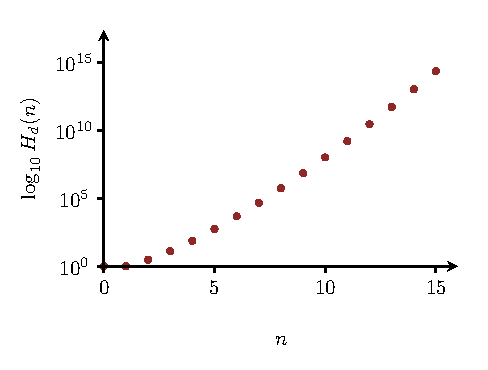
\includegraphics[width=0.75\textwidth,height=\textheight]{figures/bell/bell.pdf}

}

\caption{\label{fig-bell}The \(n\)th ordered Bell number counts the
number of ordered partitions of a finite set with \(n\) elements. As the
size of a set increases, the number of ordered partitions increases
extraordinarily quickly; even on a log scale the growth is exponential.}

\end{figure}%

That said, most practical applications consider only \textbf{atomic
decompositions} that decompose joint probability distributions as much
as possible. An atomic decomposition is defined by an atomic partition,
where each cell consists of only a single component index, \[
\mathsf{i}_{k} = \{ i_{k} \}.
\] This results in the sequence of conditional probability kernels \[
\pi(
  \mathsf{x}_{ i_{k} } \mid
  x_{ i_{k + 1} }, \ldots, x_{ i_{I} }
)
\] and the marginal distribution \[
\pi( \mathsf{x}_{ i_{I} } ).
\] Here the conditional decomposition ``peels'' off one component space
at a time in the prescribed order.

Given \(I\) component spaces, there are \(I!\) of these atomic
decompositions, each corresponding to a particular ordering of the
components. For instance, when working with the product space \[
X^{1:3} = X_{1} \times X_{2} \times X_{3},
\] we have only six unique atomic decompositions corresponding to the
partitions \begin{align*}
&{1}, {2}, {3}; \quad {1}, {3}, {2}; \quad {2}, {1}, {3};
\\
&{2}, {3}, {1}; \quad {3}, {1}, {2}; \quad {3}, {2}, {1}.
\end{align*}

\subsection{Sequential Construction of Joint Probability
Distributions}\label{sequential-construction-of-joint-probability-distributions}

Often conditional decompositions are much more useful for building up
joint distributions rather than tearing them down.

Given a partition of the component indices, we can always construct a
joint distribution by working through the index subsets in reverse. We
begin by engineering an appropriate marginal distribution \[
\pi( \mathsf{x}_{ \mathsf{i}_{K} } ).
\] over the space \(X^{ \mathsf{i}_{K} }\). Then we engineer a
conditional probability kernel, \[
\pi(
  \mathsf{x}_{ \mathsf{i}_{K - 1} } \mid
  x_{ \mathsf{i}_{k} }
)
\] over the cross sections \[
X^{ \mathsf{i}_{K - 1} } \times \{ x_{ \mathsf{i}_{K} } \}
\] before iterating and engineering a conditional probability kernel \[
\pi(
  \mathsf{x}_{ \mathsf{i}_{k} } \mid
  x_{ \cup_{k' = k + 1}^{K} \mathsf{i}_{k} }
)
\] for each subsequent cross section, \[
X^{ \mathsf{i}_{k} } \times
\{ x_{ \cup_{k' = k + 1}^{K} \mathsf{i}_{k} } \}.
\] This sequence of conditional probability kernels ``lifts'' the
initial marginal distribution into a joint distribution over the full
product space.

When the index subsets are small, the intermediate cross sections will
be low-dimensional spaces relative to the full product space. Because
engineering probabilistic objects over low-dimensional spaces is
typically much more manageable then trying to work with the entire
product space at once, this piece-wise construction is often much more
productive in practical applications.

When building off of an atomic decomposition, we will only ever have to
work with a single active component space at a time, starting with \[
\pi( \mathsf{x}_{ i_{I} } ),
\] and then proceeding to each \[
\pi(
  \mathsf{x}_{ i_{k} } \mid
  x_{ i_{k + 1} }, \ldots, x_{ i_{I} }.
)
\]

\subsection{Conditional Dependencies and
Independencies}\label{conditional-dependencies-and-independencies}

The behavior of the conditional probability distributions at any step of
a conditional decomposition, \[
\pi(
  \mathsf{x}_{ \mathsf{i}_{k} } \mid
  \tilde{x}_{ \cup_{k' = k + 1}^{K} \mathsf{i}_{k} }
)
\] can, in general, depend on the behavior in each of the remaining
component spaces, \(X_{i}\) for \[
i \in \cup_{k' = k + 1}^{K} \mathsf{i}_{k}.
\] If the conditional behavior in \(X^{ \mathsf{i}_{k} }\) varies with
the behavior in the component space \(X_{i}\), then we say that
\(X^{ \mathsf{i}_{k} }\) is \textbf{conditionally dependent} on
\(X_{i}\).

Note that this is a \emph{direct} dependency. The conditional behavior
in \(X^{ \mathsf{i}_{k} }\) may not directly depend on the behavior in a
component space \(X_{i}\). If, however, it depends on the behavior in
another component space \(X_{i'}\), and the conditional behavior in that
space depends on \(X_{i}\), then the behavior in \(X_{i}\) can
\emph{indirectly} moderate the behavior in \(X^{ \mathsf{i}_{k} }\).

These indirect dependencies are characterized by the \textbf{conditional
independencies} of a conditional decomposition. For much more on
conditional independencies in atomic conditional decompostions, see
(Bishop 2006).

The conditional dependencies of a joint probability distribution are
directly communicated by the structure of each conditional probability
kernel in a conditional decomposition. For example, if \[
\pi(
  \mathsf{x}_{ \mathsf{i}_{k} } \mid
  \tilde{x}_{ \cup_{k' = k + 1}^{K} \mathsf{i}_{k} }
)
=
\pi(
  \mathsf{x}_{ \mathsf{i}_{k} } \mid
  \tilde{x}_{i'}
)
\] then the behavior in \(X^{ \mathsf{i}_{k} }\) conditionally depends
on the behavior in only the component space \(X_{i'}\).

Alternatively, we can also communicate these conditional dependencies
with an \textbf{dependency subset} \(\mathsf{d}_{k}\) that includes all
of the relevant component indices. In general, \[
\mathsf{d}_{K} = \emptyset
\] and \[
\mathsf{d}_{k} \subseteq \cup_{k' = k + 1}^{K} \mathsf{i}_{k}.
\] Dependency subsets, however, are most informative when they include
only fewer component indices. For instance, in the above example we
would have \(\mathsf{d}_{k} = \{ i' \}\).

Conveniently, dependency subsets can be neatly organized into the
component index partition that defines a conditional decomposition in
the first place. In particular, the full structure of a conditional
decomposition can be characterized by ordered pairs of index subsets, \[
( ( \mathsf{i}_{1}, \mathsf{d}_{1}), \ldots,
  ( \mathsf{i}_{K}, \mathsf{d}_{K} ),
\] where \(\mathsf{i}_{k}\) communicates the active components at each
step while \(\mathsf{d}_{k}\) communicates the direct dependencies.

One nice feature of this more abstract characterization of conditional
dependencies is it does not depend on the precise form of the
conditional probability kernels. This allows us to, for instance, refer
to any joint model that exhibits the same conditional dependencies. Even
better, it allows us to separate the construction of a joint model into
more steps: first specifying conditional dependencies, and only
afterwards worrying about engineering the precise form of the
conditional probability kernels.

To demonstrate the use of these more abstract conditional dependencies,
let's consider the simplest possible behavior. If \[
\mathsf{d}_{k} = \emptyset
\] for all \(k\), then the behavior of every conditional probability
kernel will be completely independent of the behavior in every
subsequent component space, \[
\pi(
  \mathsf{x}_{ \mathsf{i}_{k} } \mid
  \tilde{x}_{ \cup_{k' = k + 1}^{K} \mathsf{i}_{k} }
)
=
\pi(
  \mathsf{x}_{ \mathsf{i}_{k} } \mid
  \emptyset
)
=
\pi(
  \mathsf{x}_{ \mathsf{i}_{k} }
).
\]

Any joint distribution that exhibits these conditional dependencies,
however, is an independent product of component probability
distributions in each \(X^{ \mathsf{i}_{k} }\)! When this is true for an
atomic conditional decomposition, then these joint distributions will be
independent product distributions, \[
\pi( \mathrm{d} x_{1}, \ldots, \mathrm{d} x_{I} )
=
\pi( \mathrm{d} x_{1} ) \,
\ldots \,
\pi( \mathrm{d} x_{i}  ) \,
\ldots \,
\pi( \mathrm{d} x_{I} ).
\] In other words, conditional dependencies give us yet another way to
characterize independent product distributions.

All of this said, these abstract conditional dependencies can still be a
bit ungainly to work with in practice. Fortunately, they admit a
powerful \emph{graphical} representation that we will discuss in
\textbf{Section Blah}.

\section{Product Probability Density
Functions}\label{product-probability-density-functions}

In order to anchor all of this probability theory into a concrete
foundation, we need to be able to actually implement probabilistic
calculations. To do that, we'll need to consider probability density
functions. Fortunately, product structure provides all of the
ingredients we need to construct useful joint and conditional
probability density functions.

\subsection{Product Reference
Measures}\label{product-reference-measures}

In theory, we can always try to define a reference measure directly over
a given product space. As with most product structures, however, it will
be almost always be more useful to build up a product reference measure
from component pieces. If each component space \(X_{i}\) is equipped
with a reference measure \(\nu_{i}\) that admits practical integration,
then their independent product \(\nu^{1:I}\) defines a natural reference
measure over the corresponding product space.

Provided that each of the component reference measures are
\(\sigma\)-finite, the Fubini-Tonelli theorem then allows us to evaluate
integrals with respect to \(\nu^{1:I}\) by iterating the integration
operations defined by each \(\nu_{i}\). As we discussed in
\textbf{Section Blah}, for instance, integrals with respect to a product
counting measure can be evaluated by nesting discrete sums, while
integrals with respect to a product of Lebesgue measures can often be
evaluated by nesting one-dimensional Riemann integrals.

Another powerful feature of independent product reference measures is
their disintegrations with respect to any projection function are as
well-behaved as we could hope.

Consider, for example, a subset of components, \[
\mathsf{i} \subset 1:I,
\] the corresponding projection function, \[
\varpi_{\mathsf{i}} : X^{1:I} \rightarrow X^{\mathsf{i}},
\] and a natural reference measure over the output space,
\(\nu^{ \mathsf{i} }\). Together, these objects disintegrate
\(\nu^{1:I}\) into a collection of conditional measures \[
\nu^{\varpi_{\mathsf{i}}}(
  \mathsf{x}_{\mathsf{i}^{c}} \mid x_{ \mathsf{i} }
)
\] defined over each of the cross sections \[
\varpi_{\mathsf{i}}^{-1}( x_{\mathsf{i}} )
=
X^{\mathsf{i}^{c}} \times \{ x_{\mathsf{i}} \}.
\]

Moreover, these conditional measures are equivalent to independent
product measures over the complementary components, \[
\nu^{\varpi_{\mathsf{i}}}(
  \mathsf{x}_{\mathsf{i}^{c}} \mid
  \tilde{x}_{ \mathsf{i} }
)
\cong
\nu^{ \mathsf{i}^{c} } (
  \mathsf{x}_{\mathsf{i}^{c}}
)
\] for all \[
\tilde{x}_{ \mathsf{i} } \in X^{ \mathsf{i} }.
\] This means that we can also use the Fubini-Tonelli theorem to
evaluate \emph{conditional} integrals as nested component integrals.

If we know how to integrate on each component space, then independent
product reference measures allow us to integrate on all of the relevant
product spaces and cross sections.

\subsection{Joint and Conditional Probability Density
Functions}\label{joint-and-conditional-probability-density-functions}

Once we have an independent product reference measure, the construction
of probability density functions, and consequently the evaluation of
expectation values, is immediate.

For any probability distribution \(\pi\) defined over the full product
space, we can construct the \textbf{joint probability density function},
or simply \textbf{joint density function} using the independent product
reference measure, \[
p( x_{1}, \ldots, x_{I} )
=
\frac{
  \mathrm{d} \pi
}{
  \mathrm{d} \nu^{1:I}
} ( x_{1}, \ldots, x_{I} ).
\] Given this joint density function, we can then compute joint
expectation values by nesting component integrals, for example
\begin{align*}
\mathbb{E}_{ \pi }[ g ]
& =
\int \nu_{1}( \mathrm{d} x_{1} ) \bigg[ \ldots
\\
& \quad\quad \int \nu_{i}( \mathrm{d} x_{i} ) \bigg[ \ldots
\\
& \quad\quad\quad\quad
\int \nu_{I}( \mathrm{d} x_{I} ) \,
          p( x_{1}, \ldots, x_{I} ) \,
          g( x_{1}, \ldots, x_{I} )
\\
& \hspace{18mm} \ldots \bigg]
\\
& \hspace{15mm} \ldots \bigg].
\end{align*} Provided that the joint expectation value is well-defined,
any ordering of the component integrals will yield the same answer.

Similarly, for any \(\mathsf{i} \subset 1:I\) we can construct a
\textbf{marginal probability density function}, or simply
\textbf{marginal density function}, \[
p( x_{ \mathsf{i} } )
=
\frac{
  \mathrm{d} ( \varpi_{\mathsf{i}} )_{*} \pi
}{
  \mathrm{d} \nu^{ \mathsf{i} }
} ( x_{ \mathsf{i} } ),
\] On the cross sections of any \(\mathsf{i}\) we can define
\textbf{conditional probability density functions}, or simply
\textbf{conditional density functions}, \[
p( x_{\mathsf{i}^{c}} \mid x_{ \mathsf{i} } )
=
\frac{
  \mathrm{d} \pi^{\varpi_{\mathsf{i}}}
}{
  \mathrm{d} \nu^{\varpi_{\mathsf{i}}}
} ( x_{\mathsf{i}^{c}} \mid x_{ \mathsf{i} } ).
\] The computation of marginal and conditional expectation values once
again follows from the Fubini-Tonelli theorem and the component
integration operations.

This is all a bit easier to follow when we allow for explicit
components. To that end, consider \(I = 4\) rigid real lines that form
the product space \[
X^{1:I} = \mathbb{R}^{4}.
\] Because each component space is equipped with a specific metric, we
can construct a unique Lebesgue reference measure \(\lambda_{i}\) on
each of them. The independent product of these component reference
measures defines the joint reference measure \(\lambda^{1:4}\).

This allows us to construct joint density functions, \[
p( x_{1}, x_{2}, x_{3}, x_{4} )
=
\frac{
  \mathrm{d} \pi
}{
  \mathrm{d} \nu^{1:I}
} ( x_{1}, x_{2}, x_{3}, x_{4} ),
\] and evaluate joint expectation values with nested Riemann integrals,
for instance \[
\mathbb{E}_{ \pi }[ g ]
=
\int \mathrm{d} x_{1} \, \int \mathrm{d} x_{2} \,
\int \mathrm{d} x_{3} \, \int \mathrm{d} x_{4} \,
  p( x_{1}, x_{2}, x_{3}, x_{4} ) \,
  g( x_{1}, x_{2}, x_{3}, x_{4} ).
\]

Given the component subset \[
\mathsf{i} = \{ 2, 4 \},
\] with \[
\mathsf{i}^{c} = \{ 1, 3 \},
\] we can disintegrate this joint density function into a marginal
density function, \[
p( x_{2}, x_{4} ),
\] and conditional density functions, \[
p( x_{1}, x_{3} \mid x_{2}, x_{4} ).
\] Marginal and conditional integrals are, once again, given by nesting
the appropriate component integrals.

\subsection{Decomposition and
Composition}\label{decomposition-and-composition}

In practice, we rarely if ever construct joint, marginal, and
conditional density functions separately. Instead, it's almost always
more convenient \emph{derive} them from each other.

As we saw in
\href{http://www.symplectomorphic.com/assets/chapters_html/conditional_probability_density_functions.html}{Chapter
9}, for example, a marginal density function can be derived from the a
joint density function by integrating over the cross sections, \[
p( x_{ \mathsf{i} } )
\overset{ \nu^{\mathsf{i}} }{=}
\int \nu^{\varpi_{\mathsf{i}}} ( x_{\mathsf{i}^{c}} )
p( x_{\mathsf{i}^{c}}, x_{ \mathsf{i} } ).
\] This is no longer an abstract result, however, as the conditional
integrals can now be evaluated with the Fubini-Tonelli theorem.

At the same time, the product rule relates the joint, marginal, and
conditional probability density functions together, \[
p( x_{\mathsf{i}^{c}}, x_{ \mathsf{i} } )
\overset{ \nu^{1:I} }{=}
p( x_{\mathsf{i}^{c}} \mid x_{ \mathsf{i} } ) \,
p( x_{ \mathsf{i} } ).
\] This allows us to derive any one of these objects from the other two.

Given a joint density function we can derive a marginal density function
by integrating over the cross sections, and then construct conditional
density functions from point-wise division, \[
p( x_{\mathsf{i}^{c}} \mid x_{ \mathsf{i} } )
\overset{ \nu^{1:I} }{=}
\frac{
  p( x_{\mathsf{i}^{c}}, x_{ \mathsf{i} } )
}{
  p( x_{ \mathsf{i} } ).
}
\]

To demonstrate, let's consider the product space
\(X^{1:2} = \mathbb{R}^{2}\) equipped with a multivariate Lebesgue
reference measure. This allows us to define a joint distribution through
the joint density function (Figure~\ref{fig-decomp1-joint}) \[
p( x_{1}, x_{2} )
=
\frac{
  1
}{
  2 \, \pi \,
  \sqrt{
    \sigma_{1}^{2} \, \sigma_{2}^{2} \, (1 - \rho^{2} )
  }
}
\exp \left[
  -\frac{1}{2} Q( x_{1}, x_{2} )
\right]
\] where \[
Q ( x_{1}, x_{2} )
=
\frac{
    \sigma_{2}^{2} \, x_{1}^{2}
  - 2 \, \rho \, \sigma_{1} \, \sigma_{2} \, x_{1} \, x_{2}
  + \sigma_{1}^{2} \, x_{2}^{2}
}{
  \sigma_{1}^{2} \, \sigma_{2}^{2} \, (1 - \rho^{2} ).
}
\]

The marginal density function over \(X_{1}\) is given by integrating the
joint density function over the level sets of \(\varpi_{1}\), which are
just lines where \(x_{1}\) is fixed
(Figure~\ref{fig-decomp1-level-sets}), \[
p ( x_{1} )
=
\int \mathrm{d} x_{2} \, p( x_{1}, x_{2} ).
\] After some calculus, which I've sequestered to
\hyperref[sec:app1]{Appendix A.1}, becomes a normal density function
(Figure~\ref{fig-decomp1-marginal}) \[
p ( x_{1} )
=
\text{normal} ( x_{1} \mid 0, \sigma_{1} ).
\]

Similarly, the conditional density functions become normal density
functions of their own (Figure~\ref{fig-decomp1-conditional}).
\begin{align*}
p ( x_{2} \mid x_{1} )
&=
\frac{ p ( x_{1},  x_{2} ) }{ p ( x_{1} ) }
\\
\text{normal} \left(
  x_{2} \biggm|
  \rho \frac{ \sigma_{2} }{ \sigma_{1} } x_{1},
  \sigma_{2} \sqrt{ 1 - \rho^{2} }
\right).
\end{align*}

\begin{figure}

\begin{minipage}{0.05\linewidth}
~\end{minipage}%
%
\begin{minipage}{0.45\linewidth}

\centering{

\captionsetup{labelsep=none}
\includegraphics{figures/decomp1/joint/joint.pdf}

}

\subcaption{\label{fig-decomp1-joint}}

\end{minipage}%
%
\begin{minipage}{0.45\linewidth}

\centering{

\captionsetup{labelsep=none}
\includegraphics{figures/decomp1/level_sets/level_sets.pdf}

}

\subcaption{\label{fig-decomp1-level-sets}}

\end{minipage}%
%
\begin{minipage}{0.05\linewidth}
~\end{minipage}%
\newline
\begin{minipage}{0.05\linewidth}
~\end{minipage}%
%
\begin{minipage}{0.45\linewidth}

\centering{

\captionsetup{labelsep=none}
\includegraphics{figures/decomp1/marginal/marginal.pdf}

}

\subcaption{\label{fig-decomp1-marginal}}

\end{minipage}%
%
\begin{minipage}{0.45\linewidth}

\centering{

\captionsetup{labelsep=none}
\includegraphics{figures/decomp1/conditional/conditional.pdf}

}

\subcaption{\label{fig-decomp1-conditional}}

\end{minipage}%
%
\begin{minipage}{0.05\linewidth}
~\end{minipage}%

\caption{\label{fig-decomp1}The two-dimensional real space
\(\mathbb{R}^{2}\) is a product space with rich product structure. (a) A
natural two-dimensional Lebesgue reference measure allows us to define
joint distributions by joint density functions. (b) Distinguishing the
first component \(x_{1}\) defines a projection function \(\varpi_{1}\)
whose level sets are cross sections where \(x_{1}\) is fixed. (c) The
marginal density function with respect to this projection function is
given by integrating the joint density function over the level sets of
\(\varpi_{1}\). (d) The remaining information about the joint density
function is encoded in conditional density functions defined over each
level set.}

\end{figure}%

Because of the symmetry of the joint density function, the same
calculations apply when deriving the marginal density over \(X_{2}\) and
the corresponding conditional density functions. The result there just
swaps all of the component indices (Figure~\ref{fig-decomp2})
\begin{align*}
p ( x_{2} )
&=
\text{normal} ( x_{2} \mid 0, \sigma_{2} )
\\
p ( x_{1} \mid x_{2} )
&=
\text{normal} \left(
  x_{1} \biggm|
  \rho \frac{ \sigma_{1} }{ \sigma_{2} } x_{2},
  \sigma_{1} \sqrt{ 1 - \rho^{2} }
\right).
\end{align*}

\begin{figure}

\begin{minipage}{0.05\linewidth}
~\end{minipage}%
%
\begin{minipage}{0.45\linewidth}

\centering{

\captionsetup{labelsep=none}
\includegraphics{figures/decomp2/joint/joint.pdf}

}

\subcaption{\label{fig-decomp2-joint}}

\end{minipage}%
%
\begin{minipage}{0.45\linewidth}

\centering{

\captionsetup{labelsep=none}
\includegraphics{figures/decomp2/level_sets/level_sets.pdf}

}

\subcaption{\label{fig-decomp2-level-sets}}

\end{minipage}%
%
\begin{minipage}{0.05\linewidth}
~\end{minipage}%
\newline
\begin{minipage}{0.05\linewidth}
~\end{minipage}%
%
\begin{minipage}{0.45\linewidth}

\centering{

\captionsetup{labelsep=none}
\includegraphics{figures/decomp2/marginal/marginal.pdf}

}

\subcaption{\label{fig-decomp2-marginal}}

\end{minipage}%
%
\begin{minipage}{0.45\linewidth}

\centering{

\captionsetup{labelsep=none}
\includegraphics{figures/decomp2/conditional/conditional.pdf}

}

\subcaption{\label{fig-decomp2-conditional}}

\end{minipage}%
%
\begin{minipage}{0.05\linewidth}
~\end{minipage}%

\caption{\label{fig-decomp2}We can also disintegrate the joint density
function in Figure~\ref{fig-decomp2} with respect to \(\varpi_{2}\).}

\end{figure}%

Alternatively, a marginal density function and collection of conditional
density functions together define joint density function by point-wise
multiplication, \[
p( x_{\mathsf{i}^{c}}, x_{ \mathsf{i} } )
\overset{ \nu^{1:I} }{=}
p( x_{\mathsf{i}^{c}} \mid x_{ \mathsf{i} } ) \,
p( x_{ \mathsf{i} } ).
\] Moreover, given a conditional decomposition with the active component
subsets \(\mathsf{i}_{k}\) and a sequence of conditional probability
density functions, we can apply the product rule iteratively to define
the joint probability density function \[
p( x_{1:I} )
\overset{ \nu^{1:I} }{=}
\prod_{k = 1}^{K - 1} \left[
p( x_{ \mathsf{i}_{k} } \mid
   x_{ \cup_{k' = k + 1}^{K} \mathsf{i}_{k} } )
\right] \,
p( \mathsf{i}_{K} ).
\]

For example, given the product space \[
X^{1:I} = \mathbb{R}^{4},
\] the conditional decomposition \[
( ( \{ 4 \},    \{ 1, 2, 3 \}   ),
  ( \{ 1, 3 \}, \{ 2 \}         ),
  ( \{ 2 \},    \{ \emptyset \} )
\] would yield the joint density function \[
p( x_{1}, x_{2}, x_{3}, x_{4} )
=
p( x_{4} \mid x_{1}, x_{2}, x_{3} ) \,
p( x_{1}, x_{3} \mid x_{2}  ) \,
p( x_{2}  ).
\]

Even more explicitly, consider the mixed product space \[
X^{1:2} = \mathbb{R} \times \mathbb{Z}
\] and the conditional decomposition \[
( ( \{ 2 \}, \{ 1 \}         ),
  ( \{ 1 \}, \{ \emptyset \} ).
\] Taking \[
p( x_{1} ) \propto x_{1}^{2} \, (1 - x_{1})^{2}
\] and \[
p( x_{2} \mid x_{1} )
\propto
x_{1}^{ x_{2} } \, ( 1 - x_{1} )^{10 - x_{2} }
\] gives the joint density function (Figure~\ref{fig-comp})
\begin{align*}
p( x_{1}, x_{2} )
&=
p( x_{2} \mid x_{1} ) \, p( x_{1} )
\\
&\propto
x_{1}^{ 2 + x_{2} } \, ( 1 - x_{1} )^{ 12 - x_{2} }.
\end{align*}

\begin{figure}

\begin{minipage}{0.05\linewidth}
~\end{minipage}%
%
\begin{minipage}{0.45\linewidth}

\centering{

\captionsetup{labelsep=none}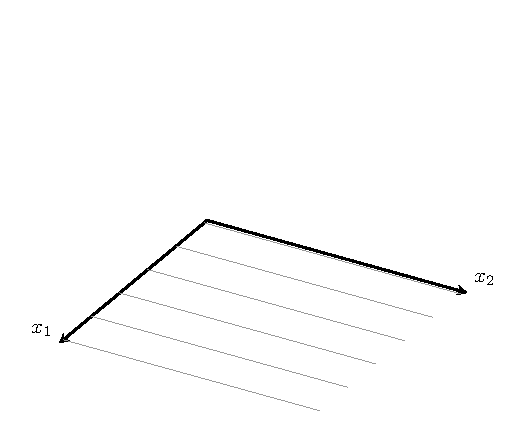
\includegraphics{figures/comp/level_sets/level_sets.pdf}

}

\subcaption{\label{fig-comp-level-sets}}

\end{minipage}%
%
\begin{minipage}{0.45\linewidth}

\centering{

\captionsetup{labelsep=none}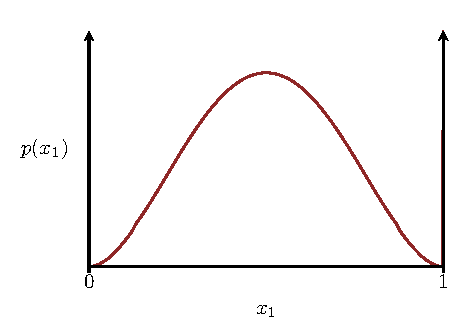
\includegraphics{figures/comp/marginal/marginal.pdf}

}

\subcaption{\label{fig-comp-marginal}}

\end{minipage}%
%
\begin{minipage}{0.05\linewidth}
~\end{minipage}%
\newline
\begin{minipage}{0.05\linewidth}
~\end{minipage}%
%
\begin{minipage}{0.45\linewidth}

\centering{

\captionsetup{labelsep=none}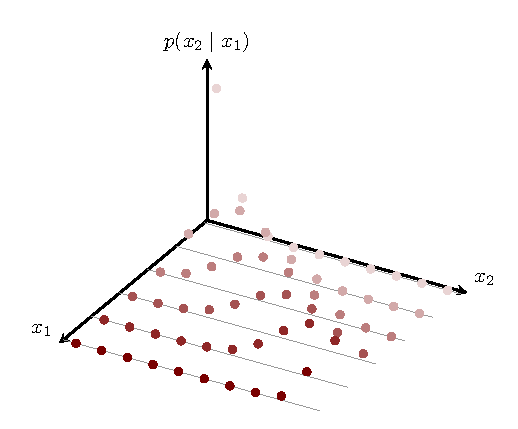
\includegraphics{figures/comp/conditional/conditional.pdf}

}

\subcaption{\label{fig-comp-conditional}}

\end{minipage}%
%
\begin{minipage}{0.45\linewidth}

\centering{

\captionsetup{labelsep=none}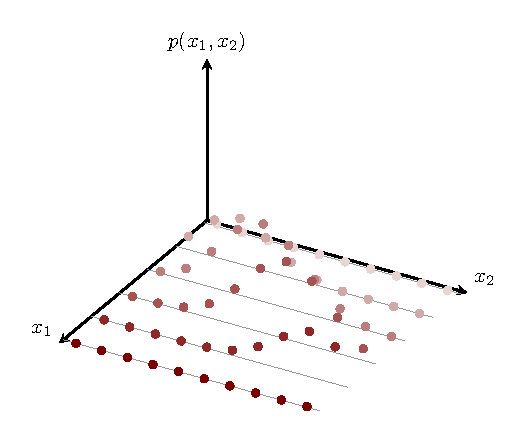
\includegraphics{figures/comp/joint/joint.pdf}

}

\subcaption{\label{fig-comp-joint}}

\end{minipage}%
%
\begin{minipage}{0.05\linewidth}
~\end{minipage}%

\caption{\label{fig-comp}Conditional decompositions provide a foundation
on which we can build up joint density functions, and hence joint
distributions. (a) A choice of conditional decomposition defines a
marginal space, here \(X_{1}\), and sequence of cross sections, here
just \(X_{2} \times \{ x_{2} \}\). (b) Any choice of marginal density
function and (c) conditional density functions defines (d) a joint
density function over the full product space.}

\end{figure}%

\subsection{The Robustness of Logarithmic Density
Functions}\label{the-robustness-of-logarithmic-density-functions}

All of this said, evaluating a joint probability density function
defined by a product of conditional density functions on a computer can
be surprisingly awkward. In particular, the multiplication of many
sequential conditional density function evaluations, each of which can
result in a number close to zero, is prone to numerical underflow.

One convenient way to avoid these numerical issues, is to not work with
probability density functions but rather work with their composition
with the natural logarithm function, \[
p( x_{1}, \ldots, x_{I} )
\mapsto
\log \circ \, p( x_{1}, \ldots, x_{I} ).
\] The logarithm of the joint density function is then given by
\emph{adding} together the logarithm of the conditional density
functions, \[
\log \circ \,  p( x_{1:I} )
\overset{ \nu^{1:I} }{=}
\sum_{k = 1}^{K - 1} \left[
\log \circ \, p( x_{ \mathsf{i}_{k} } \mid
   x_{ \cup_{k' = k + 1}^{K} \mathsf{i}_{k} } )
\right]
+ \log \circ \, p( \mathsf{i}_{K} ).
\] Because addition is a much more numerically stable operation than
multiplication, \(\log \circ \,  p( x_{1:I} )\) is much easier to
evaluate accurately on a computer.

Once we've computed this logarithmic density function, we can always
recover the joint density function whenever needed by applying the
exponential function, \[
p( x_{1}, \ldots, x_{I} )
=
\exp \left( \log \circ \, p( x_{1}, \ldots, x_{I} ) \right).
\]

\subsection{Conditioning and Partial
Evaluation}\label{conditioning-and-partial-evaluation}

The product rule allows us to immediately condition a joint probability
density function on the cross sections defined by any subset of
components \(\mathsf{i}\), \[
p( x_{\mathsf{i}^{c}} \mid x_{ \mathsf{i} } )
\overset{ \nu^{1:I} }{=}
\frac{
  p( x_{\mathsf{i}^{c}}, x_{ \mathsf{i} } )
}{
  p( x_{ \mathsf{i} } ).
}
\] In practice, however, the application of this equation is often
limited by our ability to calculate the denominator, \[
p( x_{ \mathsf{i} } )
\overset{ \nu^{\mathsf{i}} }{=}
\int \nu^{\varpi_{\mathsf{i}}} ( x_{\mathsf{i}^{c}} )
p( x_{\mathsf{i}^{c}}, x_{ \mathsf{i} } ).
\] for each \(x_{ \mathsf{i} } \in X^{ \mathsf{i} }\).

That said, when we bind \(x_{ \mathsf{i} }\) to a particular value
\(\tilde{x}_{ \mathsf{i} }\), the denominator reduces to just some
number \[
p( \tilde{x}_{ \mathsf{i} } ) \in \mathbb{R}^{+}.
\] In this case, the \emph{particular} conditional density function is,
up to proportionality, equal to the partial evaluation of the joint
density function \[
p( x_{\mathsf{i}^{c}} \mid \tilde{x}_{ \mathsf{i} } )
\overset{ \nu^{1:I} }{=}
\frac{
  p( x_{\mathsf{i}^{c}}, \tilde{x}_{ \mathsf{i} } )
}{
  p( \tilde{x}_{ \mathsf{i} } ).
}
\propto
p( x_{\mathsf{i}^{c}}, \tilde{x}_{ \mathsf{i} } ).
\]

Consequently, we don't need to be able to evaluate the marginal density
function in order to derive \emph{unnormalized} conditional density
functions. This ends up being a surprisingly powerful shortcut in many
practical applications.

Consider, for instance, a joint density function over the binary product
space \(X_{1} \times X_{2}\) defined by \[
p( x_{1}, x_{2} )
\overset{ \nu^{1:2} }{=}
p( x_{2} \mid x_{1} ) \, p( x_{1} ).
\] Because we specify \(p( x_{2} \mid x_{1} )\) directly, any
application that needs a conditional density function
\(p( x_{2} \mid \tilde{x}_{1} )\) is immediately satisfied.

The same, however, cannot be said for any application that needs an
opposing conditional density function,
\(p( x_{1} \mid \tilde{x}_{2} )\). This requires being able to calculate
\begin{align*}
p( x_{1} \mid \tilde{x}_{2} )
&=
\frac{
  p( x_{1}, \tilde{x}_{2} )
}{
  p( \tilde{x}_{2} )
}
\\
&=
\frac{
  p( x_{1}, \tilde{x}_{2} )
}{
  \int \nu_{1}( \mathrm{d} x_{1}) p( x_{1}, \tilde{x}_{2} ).
}
\end{align*}

If we cannot evaluate the normalizing integral, then we cannot construct
\(p( x_{1} \mid \tilde{x}_{2} )\). That said, if the normalization is
irrelevant, then we can skip the normalizing integral entirely, \[
p( x_{1} \mid \tilde{x}_{2} )
\overset{ \nu^{1:I} }{\propto}
p( x_{1}, \tilde{x}_{2} ).
\]

One circumstance where the marginal density function can't be neglected
is when we want to compare two conditional distributions to each other.
The Radon-Nikodym derivative between two conditional distributions is
given by the ratio of their conditional density functions. Using the
product rule, we can write this ratio as \begin{align*}
\frac{
  p( x_{1} \mid \tilde{x}_{2} )
}{
  p( x_{1} \mid \tilde{x}'_{2} )
}
&\overset{ \nu^{1:2} }{=}
\frac{
  p( x_{1}, \tilde{x}_{2} )
}{
  p( \tilde{x}_{2} )
}
\frac{
  p( \tilde{x}'_{2} )
}{
  p( x_{1}, \tilde{x}'_{2} )
}
\\
&\overset{ \nu^{1:2} }{=}
\frac{
  p( x_{1}, \tilde{x}_{2} )
}{
  p( x_{1}, \tilde{x}'_{2} )
}
\frac{
  p( \tilde{x}'_{2} )
}{
  p( \tilde{x}_{2} ).
}
\end{align*} In this case, the ratio of the marginal density function
evaluations is critical to an accurate comparison.

\section{Directed Graphical Models}\label{directed-graphical-models}

So far we have seen conditional decompositions defined explicitly, as a
collection of active and dependency subsets, and implicitly, by writing
out a sequence of conditional density functions and tailing marginal
density function. In this section we will be introduced to a
\emph{visual} representation of conditional decompositions that neatly
complements these methods.

\subsection{Directed Acyclic Graphs}\label{directed-acyclic-graphs}

A \textbf{graph} is a collection of \textbf{nodes} with \textbf{edges}
connected certain pairs of nodes. Typically nodes represent mathematical
objects and edges the relationships, or lack thereof, between those
objects.

\textbf{Directed graphs} (Bishop 2006) distinguish between edges that
originate from one node and terminate in another, and vice versa. The
structure of a directed graph is particularly straightforward to
visualize, with two-dimensional shapes representing each node and
one-dimensional arrows the directed edges between them
(Figure~\ref{fig-dgm1}).

\begin{figure}

\centering{

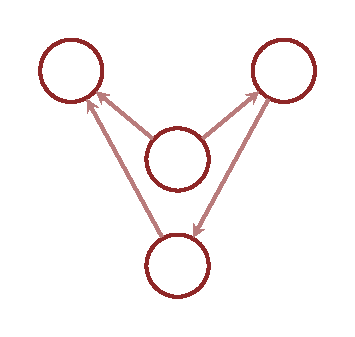
\includegraphics[width=0.33\textwidth,height=\textheight]{figures/dgms/1/dg.pdf}

}

\caption{\label{fig-dgm1}Directed graphs are typically visualized using
shapes to represent each node and arrows to represent the edges between
them. When the nodes of a directed graph are labeled, we can also label
the shapes accordingly.}

\end{figure}%

The nodes at which a directed edge originates is referred to as the
\textbf{parent} of the node at which the edge terminates. Similarly, the
terminating node is referred to as a \textbf{child} of originating node
(Figure~\ref{fig-dgm2}). This familial language motivates a variety of
related vocabulary, such as referring to two nodes that share a common
parent as siblings.

\begin{figure}

\centering{


\includegraphics[width=0.25\textwidth,height=\textheight]{figures/dgms/2/dg.pdf}

}

\caption{\label{fig-dgm2}Two nodes connected by a directed edge are
referred to as the parent and child of each other. This terminology
allows us to compact describe relationships between nodes in a directed
graph.}

\end{figure}%

A sequence of directed edges connecting parent nodes to child nodes
defines a \textbf{path} through the graph. In general, these paths can
circle back on themselves, forming \textbf{cycles}
(Figure~\ref{fig-dgm3}). Directed graphs that do not exhibit any cycles
(Figure~\ref{fig-dgm4}) are known as \textbf{directed acyclic graphs},
or often just \textbf{DAGs} for short.

\begin{figure}

\begin{minipage}{0.15\linewidth}
~\end{minipage}%
%
\begin{minipage}{0.35\linewidth}

\centering{

\captionsetup{labelsep=none}
\includegraphics{figures/dgms/3/dg.pdf}

}

\subcaption{\label{fig-dgm3}}

\end{minipage}%
%
\begin{minipage}{0.35\linewidth}

\centering{

\captionsetup{labelsep=none}
\includegraphics{figures/dgms/4/dg.pdf}

}

\subcaption{\label{fig-dgm4}}

\end{minipage}%
%
\begin{minipage}{0.15\linewidth}
~\end{minipage}%

\caption{\label{fig-dags}(a) Cycles in a directed graph are formed by
paths of edges that connect back on themselves. (b) In a directed
acyclic graph, each path originates and terminates at a distinct node.}

\end{figure}%

Because of the lack of cycles, directed acyclic graphs exhibit a
well-defined notion of directionality (Figure~\ref{fig-dgm5}). On one
side of the graph we have \textbf{root nodes} with no parents, and on
the other we have \textbf{leaf nodes} with no children.

\begin{figure}

\centering{


\includegraphics[width=0.75\textwidth,height=\textheight]{figures/dgms/5/dg.pdf}

}

\caption{\label{fig-dgm5}Directed acyclic graph can be arranged in a
natural direction, starting with root nodes who have no parents and leaf
nodes who have no children.}

\end{figure}%

Although visualizations of directed graphs don't technically have to
respect this directionality, they tend to be more effective when they
do. That said, there is no universal convention for whether root notes
should be on the top, bottom, left, or right of a visualization. We are
free to pick whichever convention is most convenient, provided that we
maintain that convention consistently.

\subsection{Graphical Models of Atomic Conditional
Decompositions}\label{graphical-models-of-atomic-conditional-decompositions}

Conveniently, every atomic conditional decomposition defines a unique
directed acyclic graph, which can then be used to visualize the
conditional structure. A conditional decomposition represented by a
directed acyclic graph is known as a \textbf{directed graphical model},
or sometimes just \textbf{DGM} for short.

Consider, for example, the atomic conditional decomposition \[
( ( \{ i_{1} \}, \mathsf{d}_{1} ), \quad
  \ldots, \quad
  ( \{ i_{I} \}, \mathsf{d}_{I} ) ).
\] Each subset of active components, \[
\mathsf{i}_{k} = \{ i_{k} \}
\] can be represented by a node labeled with the corresponding component
variable. At the same time, each pair
\(( ( \{ i_{k} \}, \mathsf{d}_{k} )\) defines a collection of directed
edges, each of which originates from one of the nodes representing the
elements of \(\mathsf{d}_{k}\) and terminating at the node representing
\(i_{k}\).

To demonstrate, let's build a graphical model for a joint distribution
defined over the product space \[
X = X_{1} \times X_{2} \times X_{3} \times X_{4}
\] with the conditional decomposition \[
( ( \{ 4 \}, \{ 1, 3 \}      ),  \quad
  ( \{ 3 \}, \{ 1, 2 \}      ),  \quad
  ( \{ 1 \}, \{ 2 \}         ),  \quad
  ( \{ 2 \}, \{ \emptyset \} )  ).
\] Equivalently, we can interpret this as building a graphical model for
the density function decomposition \begin{align*}
p( x_{1}, x_{2}, x_{3}, x_{4} )
&= \;\,
p( x_{4} \mid x_{1}, x_{3} )
\\
&\quad \cdot
p( x_{3} \mid x_{1}, x_{2} )
\\
&\quad \cdot
p( x_{1} \mid x_{2} )
\\
&\quad \cdot
p( x_{2} ).
\end{align*}

Each of the four component spaces defines a node in the corresponding
graphical model (Figure~\ref{fig-dgm6a}). Because the behavior in
\(X_{4}\) depends on the behavior in \(X_{1}\) and \(X_{3}\), we then
place two directed edges from the nodes representing \(X_{1}\) and
\(X_{3}\) to the node representing \(X_{4}\) (Figure~\ref{fig-dgm6b}).
Next, we place two directed edges that terminate at the node
representing \(X_{3}\), and one that terminates at the node representing
\(X_{1}\) (Figure~\ref{fig-dgm6c}). Finally, we place one last directed
edge from the node representing \(X_{2}\) to the node representing
\(X_{1}\) (Figure~\ref{fig-dgm6d}). The behavior in \(X_{2}\) is
independent of the behavior in any of the other component spaces;
consequently, there are no more directed edges to place.

\begin{figure}

\begin{minipage}{0.15\linewidth}
~\end{minipage}%
%
\begin{minipage}{0.35\linewidth}

\centering{

\captionsetup{labelsep=none}
\includegraphics{figures/dgms/6a/dg.pdf}

}

\subcaption{\label{fig-dgm6a}}

\end{minipage}%
%
\begin{minipage}{0.35\linewidth}

\centering{

\captionsetup{labelsep=none}
\includegraphics{figures/dgms/6b/dg.pdf}

}

\subcaption{\label{fig-dgm6b}}

\end{minipage}%
%
\begin{minipage}{0.15\linewidth}
~\end{minipage}%
\newline
\begin{minipage}{0.15\linewidth}
~\end{minipage}%
%
\begin{minipage}{0.35\linewidth}

\centering{

\captionsetup{labelsep=none}
\includegraphics{figures/dgms/6c/dg.pdf}

}

\subcaption{\label{fig-dgm6c}}

\end{minipage}%
%
\begin{minipage}{0.35\linewidth}

\centering{

\captionsetup{labelsep=none}
\includegraphics{figures/dgms/6d/dg.pdf}

}

\subcaption{\label{fig-dgm6d}}

\end{minipage}%
%
\begin{minipage}{0.15\linewidth}
~\end{minipage}%

\caption{\label{fig-dags}Graphical models are straightforward to build
for atomic conditional decompositions. (a) After placing nodes for each
component space, (b-d) we work down the conditional decomposition,
placing directed arrows between every component node and its
dependencies.}

\end{figure}%

For this conditionald decomposition, the node representing \(X_{4}\) is
the lone leaf node. At the same time, the node representing \(X_{2}\) is
the only root node.

The more coupled the behavior in the component spaces are to each other,
the more directed edges the corresponding graphical model will feature.
Often the most informative aspect of a graphical model is the
\emph{absence} of directed edges.

\subsection{Graphical Models of More General Conditional
Decompositions}\label{graphical-models-of-more-general-conditional-decompositions}

Unfortunately, once we move away from atomic conditional decompositions,
graphical modeling becomes a little bit more complicated. The problem is
that not every general conditional decompositions defines a distinct
directed acyclic graph. In other words, some graphical models will be
ambiguous.

To see what can go wrong, let's go back to the product space \[
X = X_{1} \times X_{2} \times X_{3} \times X_{4},
\] but now consider the conditional decomposition \[
( ( \{ 4 \},    \{ 1, 2 \}      ), \quad
  ( \{ 1, 3 \}, \{ 2 \}         ), \quad
  ( \{ 2 \},    \{ \emptyset \} )  ).
\] Again, we can equivalently interpret this as the density function
decomposition \[
p( x_{1}, x_{2}, x_{3}, x_{4} )
=
p( x_{4} \mid x_{1}, x_{2} ) \,
p( x_{1}, x_{3} \mid x_{2} ) \,
p( x_{2} ).
\]

Here we'll need a directed edge to represent the conditional dependence
of the behavior in \(X_{4}\) on the behavior in \(X_{1}\). There is no
node, however, that represents just \(X_{1}\). Instead we have a node
that represents both \(X_{1}\) and \(X_{3}\).

One option is to add a directed edge that originates from the node
representing \(X_{1} \times X_{3}\) and terminates at the node
representing \(X_{4}\) (Figure~\ref{fig-dgm7}). This approach, however,
would have us add the same exact edge if the behavior in \(X_{4}\)
conditionally depended on \(X_{3}\) or \(X_{1} \times X_{3}\)!

\begin{figure}

\centering{


\includegraphics[width=0.75\textwidth,height=\textheight]{figures/dgms/7/dg.pdf}

}

\caption{\label{fig-dgm7}Not every non-atomic conditional decomposition
translates to a unique graphical model. The graphical model here is
consistent with three different conditional decompositions.}

\end{figure}%

In other words, this graphical model represents three distinct
conditional decompositions, \begin{align*}
& ( ( \{ 4 \},    \{ 1, 2 \}   ), \quad
    ( \{ 1, 3 \}, \{ 2 \}         ), \quad
    ( \{ 2 \},    \{ \emptyset \} )  )
\\
& ( ( \{ 4 \},    \{ 1, 3 \}   ), \quad
    ( \{ 1, 3 \}, \{ 2 \}         ), \quad
    ( \{ 2 \},    \{ \emptyset \} )  )
\\
& ( ( \{ 4 \},    \{ 1, 2, 3 \}   ), \quad
    ( \{ 1, 3 \}, \{ 2 \}         ), \quad
    ( \{ 2 \},    \{ \emptyset \} )  ),
\end{align*} at the same time. Without additional information, there
would be no way to know which of these conditional decomposition was
intended from the graphical model alone.

Fortunately, it's not \emph{too} difficult to characterize a more
general class of conditional decompositions that correspond to unique
graphical models. The key is to consider only those conditional
decompositions where each dependency subset \(\mathsf{d}_{k}\) is the
union of some number of active component subsets \(\mathsf{i}_{k'}\), \[
\mathsf{d}_{k} = \bigcup_{k'} \mathsf{i}_{k'}.
\] In this case, the behavior in \(X^{ \mathsf{i}_{k} }\) will always
depend on \emph{all} of the component spaces in a node representing
\(X^{ \mathsf{i}_{k'} }\) or \emph{none} of them. Consequently, each
directed edge will always have a unique origin and terminus.

For instance, of the three conditional decompositions that we considered
above, only \[
( ( \{ 4 \},    \{ 1, 2, 3 \}   ), \quad
  ( \{ 1, 3 \}, \{ 2 \}         ), \quad
  ( \{ 2 \},    \{ \emptyset \} )  )
\] satisfies this disambiguating criteria. The other two conditional
decompositions would have to be excluded to avoid any ambiguity.

A simpler way to interpret this disambiguating criteria is that is
reinterprets the components of the product space to be not the
\(X_{i}\), \[
X = \times_{i = 1}^{I} X_{i},
\] but rather the \(X^{ \mathsf{i}_{k} }\), \[
X = \times_{k = 1}^{K} X^{ \mathsf{i}_{k} }.
\] Any conditional decomposition built around these composite components
will necessarily treat each \(X^{ \mathsf{i}_{k} }\) uniformly.

Many references avoid this awkwardness entirely by using graphical
models for only atomic conditional decompositions. That said, more
general graphical modeling can be extremely useful in practice, even if
used only informally. In this book, I will be relatively generous with
my applications of graphical modeling, taking care to respect the
disambiguating criteria.

\subsection{Bells and Whistles}\label{bells-and-whistles}

The nodes and edges in directed graphical models convey a wealth of
information. We can, however, pack even more information into directed
graphical models by augmenting this basic graph structure with some
special features.

\subsubsection{Auxiliary Nodes}\label{auxiliary-nodes}

Many applications consider joint distributions whose behavior depends on
the behavior of auxiliary spaces that are not equipped with any
probabilistic structure of their own. In other words, these joint
distributions are \emph{parameterized} by the configuration of the
auxiliary spaces.

These non-probabilistic dependencies can be represented in graphical
models by introducing multiple types of nodes, one to represent the
probabilistic spaces and one to represent the auxiliary spaces. I like
to use \emph{rounded} shapes to represent probabilistic nodes and
\emph{rectangular} shapes to represent auxiliary nodes.

For instance, the conditional structure of \begin{align*}
p( x_{1}, x_{2}, x_{3}, x_{4}; y )
&= \;\,
p( x_{4} \mid x_{1}, x_{3} )
\\
&\quad \cdot
p( x_{1} \mid x_{3}; y )
\\
&\quad \cdot
p( x_{3} \mid x_{2} )
\\
&\quad \cdot
p( x_{2} )
\end{align*} can be represented by the graphical model in
Figure~\ref{fig-dgm8}.

\begin{figure}

\centering{


\includegraphics[width=0.75\textwidth,height=\textheight]{figures/dgms/8/dg.pdf}

}

\caption{\label{fig-dgm8}Rectangular nodes communicate non-probabilistic
dependencies in joint probability distributions. Here the conditional
density functions \(p( x_{1} \mid x_{3}; y )\) are parameterized by the
configuration of a non-probabilistic space, \(y \in Y\).}

\end{figure}%

\subsubsection{Pushforward Nodes}\label{pushforward-nodes}

Sometimes the behavior of a component space depends on the behavior of
other component spaces through only the output of some intermediate
function. For instance, instead of \begin{align*}
p( x_{1}, x_{2}, x_{3}, x_{4}; y )
&= \;\,
p( x_{4} \mid x_{1}, x_{3} )
\\
&\quad \cdot
p( x_{1} \mid x_{3}; y )
\\
&\quad \cdot
p( x_{3} \mid x_{2} )
\\
&\quad \cdot
p( x_{2} )
\end{align*} we might have \begin{align*}
p( x_{1}, x_{2}, x_{3}, x_{4}; y )
&= \;\,
p( x_{4} \mid f( x_{1}, x_{3} ) )
\\
&\quad \cdot
p( x_{1} \mid x_{3}; y )
\\
&\quad \cdot
p( x_{3} \mid x_{2} )
\\
&\quad \cdot
p( x_{2} ).
\end{align*} In this case, the behavior in \(X_{4}\) doesn't directly
depend on the behavior in \(X_{1} \times X_{3}\), but rather the
behavior in \(X_{1} \times X_{3}\) pushed forward through \(f\).

One way to communicate these functional dependencies in a graphical
model is to introduce an explicit variable for the function output,
\begin{align*}
p( x_{1}, x_{2}, x_{3}, x_{4}; y )
&= \;\,
p( x_{4} \mid y = f(x_{1}, x_{3}) )
\\
&\quad \cdot
p( x_{1} \mid x_{3}; y )
\\
&\quad \cdot
p( x_{3} \mid x_{2} )
\\
&\quad \cdot
p( x_{2} ),
\end{align*} and then represent that variable with its own node. To
avoid any ambiguity, however, we'll need to decorate this node
differently from the component nodes. I like to use dashed borders
(Figure~\ref{fig-dgm9})

\begin{figure}

\centering{


\includegraphics[width=0.75\textwidth,height=\textheight]{figures/dgms/9/dg.pdf}

}

\caption{\label{fig-dgm9}Dashed, circular nodes represent the output of
functions that depend on components variables. We can interpret these
nodes as modeling the pushforward distribution along the intermediate
function.}

\end{figure}%

\subsubsection{Conditioned Nodes}\label{conditioned-nodes}

Some applications are less concerned with a given joint distribution
than certain conditional distributions derived from that joint
distribution when we bind particular component variables to particular
values.

Once we have a graphical model for the joint distribution, this
conditioning process is straightforward to visualize by adding a
distinct decoration to the nodes corresponding to the bound variables. A
common convention is to fully color these nodes.

For example, let's say that we start with the joint distribution defined
by the probability density functions (Figure~\ref{fig-dgm10a})
\begin{align*}
p( x_{1}, x_{2}, x_{3}, x_{4} )
&= \;\,
p( x_{4} \mid x_{1}, x_{3} )
\\
&\quad \cdot
p( x_{1} \mid x_{3} )
\\&\quad \cdot
p( x_{3} \mid x_{2} )
\\
&\quad \cdot
p( x_{2} ),
\end{align*} but we are interested in the conditional distribution
defined by \[
p( x_{2}, x_{3} \mid \tilde{x}_{1}, \tilde{x}_{4} )
=
\frac{
  p( \tilde{x}_{1}, x_{2}, x_{3}, \tilde{x}_{4} )
}{
  p( \tilde{x}_{1}, \tilde{x}_{4} ).
}
\] We can visualize this particular conditioning by coloring in the
nodes representing \(X_{1}\) and \(X_{4}\) (Figure~\ref{fig-dgm10b}).

\begin{figure}

\begin{minipage}{0.05\linewidth}
~\end{minipage}%
%
\begin{minipage}{0.45\linewidth}

\centering{

\captionsetup{labelsep=none}
\includegraphics{figures/dgms/10a/dg.pdf}

}

\subcaption{\label{fig-dgm10a}}

\end{minipage}%
%
\begin{minipage}{0.45\linewidth}

\centering{

\captionsetup{labelsep=none}
\includegraphics{figures/dgms/10b/dg.pdf}

}

\subcaption{\label{fig-dgm10b}}

\end{minipage}%
%
\begin{minipage}{0.05\linewidth}
~\end{minipage}%

\caption{\label{fig-dgm10}The various conditional distributions that we
can derive from a joint distribution can be represented by (a) taking
the graphical model for the joint distribution and (b) coloring in the
nodes representing the components being bound to particular values.}

\end{figure}%

\subsubsection{Plate Notation}\label{plate-notation}

Some conditional patterns are sufficiently common that it's useful to
introduce graphical shorthands that allow for more compact
visualizations.

Consider, for example, the product space \(X = X^{1:5}\), and the
conditional decomposition \[
( ( \{ 1 \}, \{ 5 \} ), \quad
  ( \{ 2 \}, \{ 5 \} ), \quad
  ( \{ 3 \}, \{ 5 \} ), \quad
  ( \{ 4 \}, \{ 5 \} ), \quad
  ( \{ 5 \}, \{ \emptyset \} )  ),
\] or, equivalently, the sequence of probability density functions
\begin{align*}
p( x_{1}, x_{2}, x_{3}, x_{4}, x_{5} )
&= \;\,
p( x_{1} \mid x_{5} )
\\
&\quad \cdot
p( x_{2} \mid x_{5} )
\\
&\quad \cdot
p( x_{3} \mid x_{5} )
\\
&\quad \cdot
p( x_{4} \mid x_{5} )
\\
&\quad \cdot
p( x_{5} ).
\end{align*}

This particular conditional structure results in a fan-like graphical
model (Figure~\ref{fig-dgm11}), which can take up a lot of visual space.
We can make the graphical model a bit more compact, however, by packing
the first four nodes together into a single \textbf{plate} that
represents their common dependence on the fifth node.

\begin{figure}

\begin{minipage}{0.05\linewidth}
~\end{minipage}%
%
\begin{minipage}{0.45\linewidth}

\centering{

\captionsetup{labelsep=none}
\includegraphics{figures/dgms/11/dg.pdf}

}

\subcaption{\label{fig-dgm11}}

\end{minipage}%
%
\begin{minipage}{0.45\linewidth}

\centering{

\captionsetup{labelsep=none}
\includegraphics{figures/dgms/12/dg.pdf}

}

\subcaption{\label{fig-dgm12}}

\end{minipage}%
%
\begin{minipage}{0.05\linewidth}
~\end{minipage}%

\caption{\label{fig-comp}(a) Conditional dependencies where many subsets
of active components depend on one, and only one, other subset of
components, result in fan-like graphical models. (b) These graphical
models can be visually compressed by packing the dependent nodes into a
single plate.}

\end{figure}%

This plate notation is especially useful when we have an arbitrary
number of component spaces whose behavior conditionally depends on the
same component spaces. For instance, we might have the product space
\(X = X^{1:I} \times X_{I + 1}\) and a joint distribution built up from
the conditional decomposition \[
p( x_{1}, \ldots, x_{I + 1} )
=
\left[
  \prod_{i =  1}^{I} p( x_{i} \mid x_{I + 1} )
\right] \,
p ( x_{I + 1} ).
\]

We can try to construct heuristic visualizations to represent the
arbitrary number of nodes (Figure~\ref{fig-dgm13}), but the plate
notation allow us to visualize this structure exactly
(Figure~\ref{fig-dgm14}).

\begin{figure}

\begin{minipage}{0.05\linewidth}
~\end{minipage}%
%
\begin{minipage}{0.45\linewidth}

\centering{

\captionsetup{labelsep=none}
\includegraphics{figures/dgms/13/dg.pdf}

}

\subcaption{\label{fig-dgm13}}

\end{minipage}%
%
\begin{minipage}{0.45\linewidth}

\centering{

\captionsetup{labelsep=none}
\includegraphics{figures/dgms/14/dg.pdf}

}

\subcaption{\label{fig-dgm14}}

\end{minipage}%
%
\begin{minipage}{0.05\linewidth}
~\end{minipage}%

\caption{\label{fig-comp}(a) Graphical models with an arbitrary number
of nodes are awkward to visualize. (b) When applicable, plates avoid
this awkwardness entirely.}

\end{figure}%

Plates can also be nested to accommodate \emph{hierarchical conditional
dependencies}

\begin{figure}

\begin{minipage}{0.15\linewidth}
~\end{minipage}%
%
\begin{minipage}{0.70\linewidth}

\centering{

\captionsetup{labelsep=none}
\includegraphics{figures/dgms/15/dg.pdf}

}

\subcaption{\label{fig-dgm15}}

\end{minipage}%
%
\begin{minipage}{0.15\linewidth}
~\end{minipage}%
\newline
\begin{minipage}{0.15\linewidth}
~\end{minipage}%
%
\begin{minipage}{0.70\linewidth}

\centering{

\captionsetup{labelsep=none}
\includegraphics{figures/dgms/16/dg.pdf}

}

\subcaption{\label{fig-dgm16}}

\end{minipage}%
%
\begin{minipage}{0.15\linewidth}
~\end{minipage}%

\caption{\label{fig-comp}(a) Nested hierarchies of conditional
dependencies can also be compactly visualized by (b) nested plates
within other plates.}

\end{figure}%

\subsection{Subtleties and
Limitations}\label{subtleties-and-limitations}

Directed graphical models can be a powerful tool for communicating the
structure of conditional decompositions in practice, especially as a
complement to explicit probability density functions. That said,
directed graphical models are without their subtleties and limitations
that require some care.

For instance, directed graphical models communicate the structure of a
particular \emph{conditional decomposition}, not a particular
\emph{joint distribution}. The same joint distribution under different
conditional decompositions will result in different graphical models. At
the same time, different joint distributions with the same conditional
dependencies will correspond to the same graphical model, just with
differences in the conditional distributions and/or marginal
distribution.

In other words, graphical models does no completely specify joint
distributions. Instead it defines a kind of mathematical ``armature''
around which we can build up a joint distribution with the choice of
particular conditional and marginal probability distributions. In order
to communicate those choices, we need to complement a graphical model
with additional information.

Another potential issue is that transforming a joint distribution will,
in general, transform the corresponding graphical model. Transformations
that preserve the product structure of a space will, by definition, also
preserve the structure of conditional decompositions, and hence the
structure of of graphical models. For instance, we can freely transform
individual component spaces without affecting the graphical modeling
representation. On the other hand, transformations that reorder the
component spaces or mix them together will usually change the
conditional decomposition, and hence the corresponding graphical model.

One of the more frustrating aspects of directed graphical models is that
they can struggle to effectively communicate certain operations.

Consider, for example, the joint distribution defined by the density
function decomposition \begin{align*}
p( x_{1}, \ldots, x_{6}  )
&= \;\,
p ( x_{1} \mid x_{4} - x_{6} )
\\&\quad \cdot
p ( x_{2} \mid x_{6} - x_{5} )
\\
&\quad \cdot
p ( x_{3} \mid x_{5} - x_{4} )
\\
&\quad \cdot
p ( x_{4} ) \,
p ( x_{5} ) \,
p ( x_{6} ).
\end{align*}

A graphical model using only six nodes, one for each \(X_{i}\), can be
confused with a more general conditional dependencies
(Figure~\ref{fig-dgm17}), \begin{align*}
p( x_{1}, \ldots, x_{6}  )
&= \;\,
p ( x_{1} \mid x_{4}, x_{6} )
\\&\quad \cdot
p ( x_{2} \mid x_{5},  x_{6} )
\\
&\quad \cdot
p ( x_{3} \mid x_{4}, x_{5} )
\\
&\quad \cdot
p ( x_{4} ) \,
p ( x_{5} ) \,
p ( x_{6} ).
\end{align*}

We can capture the conditional dependence on the differences with
pushforward nodes (Figure~\ref{fig-dgm17}), but the overlapping arrows
can be difficult to parse. Moreover, the parsing becomes only more
difficult as we add more nodes that also depend on differences between
\(x_{4}\), \(x_{5}\), and \(x_{6}\).

Another possibility is to employ plate notation
(Figure~\ref{fig-dgm19}). The problem with this approach, however, is
that each \(y_{i}\) doesn't depend on \(x_{4}\), \(x_{5}\), and
\(x_{6}\) all at the same time. Consequently, this plate diagram is
fundamentally ambiguous as well.

\begin{figure}

\begin{minipage}{0.01\linewidth}
~\end{minipage}%
%
\begin{minipage}{0.33\linewidth}

\centering{

\captionsetup{labelsep=none}
\includegraphics{figures/dgms/17/dg.pdf}

}

\subcaption{\label{fig-dgm17}}

\end{minipage}%
%
\begin{minipage}{0.33\linewidth}

\centering{

\captionsetup{labelsep=none}
\includegraphics{figures/dgms/18/dg.pdf}

}

\subcaption{\label{fig-dgm18}}

\end{minipage}%
%
\begin{minipage}{0.33\linewidth}

\centering{

\captionsetup{labelsep=none}
\includegraphics{figures/dgms/19/dg.pdf}

}

\subcaption{\label{fig-dgm19}}

\end{minipage}%
%
\begin{minipage}{0.01\linewidth}
~\end{minipage}%

\caption{\label{fig-comp}Some conditional decompositions are just
awkward to to represent with graphical models. Consider, for example, a
joint density function built up from the conditional density functions
\(p( x_{1} \mid x_{4} - x_{6} )\), \(p( x_{2} \mid x_{6} - x_{5} )\),
and \(p( x_{3} \mid x_{5} - x_{4} )\). (a) The immediate graphical model
doesn't communicate the particular dependence on differences. (b)
Introducing pushforward nodes helps, but at the expense of a much busier
graphical model. (c) Using plates results in a more elegant graphical
model, but requires introducing conditional indices \(j_{i}\) and
\(k_{i}\) whose behavior is left ambiguous.}

\end{figure}%

All of this is to say that graphical models are not always the best tool
for communicating conditional dependencies. Sometimes a probability
density function decomposition is just more effective. Other times we
might need to reach for other representations, such as
\emph{probabilistic programming}. This will be a topic for a future
chapter.

\section{Bayes' Theorem}\label{bayes-theorem}

Given a subset of components, we can decompose a joint distribution two
different ways. The conditional probability kernel and a tailing
marginal distribution from each of these decompositions, however, are
intimately related.

Consider the complementary component subsets \[
\mathsf{i} \subset \{ 1, \ldots, I \}
\] and \[
\mathsf{i}^{c} \subset \{ 1, \ldots, I \}.
\] The partition \[
( \mathsf{i}^{c}, \mathsf{i}  )
\] defines the conditional probability kernel \[
\pi^{\varpi_{\mathsf{i}}}(
  \mathsf{x}_{\mathsf{i}^{c}} \mid
  x_{ \mathsf{i} }
)
\] and the marginal probability distribution \[
( \varpi_{\mathsf{i}} )_{*} \pi.
\] At the same time, the permuted partition \[
( \mathsf{i},  \mathsf{i}^{c} )
\] defines the conditional probability kernel \[
\pi^{\varpi_{ \mathsf{i}^{c} }}(
  \mathsf{x}_{\mathsf{i}} \mid
  x_{ \mathsf{i}^{c} }
)
\] and the marginal probability distribution \[
( \varpi_{ \mathsf{i}^{c} } )_{*} \pi.
\]

Each conditional probability distribution in the conditional probability
kernel of the \emph{first} decomposition is defined on a cross section,
\[
X^{\mathsf{i}^{c}} \times \{ x_{\mathsf{i}} \},
\] For fixed \(x_{\mathsf{i}}\), this cross section is equivalent to the
product space \[
X^{\mathsf{i}^{c}}.
\] This, however, is exactly the space over which the marginal
probability distribution in the \emph{second} decomposition is defined.
Consequently, we can define Radon-Nikodym derivatives between these
objects, \[
\frac{
  \mathrm{d} \pi^{ \varpi_{\mathsf{i}} }
}{
  \mathrm{d} ( \varpi_{ \mathsf{i}^{c} } )_{*} \pi
}
( x_{ \mathsf{i}^{c} } \mid
  x_{ \mathsf{i} } ).
\]

Similarly, we can construct Radon-Nikodym derivatives between each
conditional probability distribution in the \emph{second} decomposition
and the marginal probability distribution in the first decomposition, \[
\frac{
  \mathrm{d} \pi^{ \varpi_{ \mathsf{i}^{c} } }
}{
  \mathrm{d} ( \varpi_{ \mathsf{i} } )_{*} \pi
}
( x_{ \mathsf{i} } \mid
  x_{ \mathsf{i}^{c} } ).
\]

In order for the two decompositions to define the same joint probability
distribution, these Radon-Nikodym derivatives have to be almost always
equal, \[
\frac{
  \mathrm{d} \pi^{ \varpi_{\mathsf{i}} }
}{
  \mathrm{d} ( \varpi_{ \mathsf{i}^{c} } )_{*} \pi
}
( x_{ \mathsf{i}^{c} } \mid
  x_{\mathsf{i}} )
\overset{ \pi }{=}
\frac{
  \mathrm{d} \pi^{ \varpi_{ \mathsf{i}^{c} } }
}{
  \mathrm{d} ( \varpi_{ \mathsf{i} } )_{*} \pi
}
( x_{ \mathsf{i} } \mid
  x_{ \mathsf{i}^{c} } ).
\]

The identification between these Radon-Nikodym derivatives admits a
particularly compelling interpretation. Consider the conditional
expectation \[
\int
\pi^{ \varpi_{ \mathsf{i}^{c} } } (
  \mathrm{d} x_{ \mathsf{i} } \mid
  \tilde{x}_{ \mathsf{i}^{c} }
) \,
g ( x_{ \mathsf{i} } ).
\] Using Radon-Nikodym derivatives, we can compute this conditional
expectation as a complementary marginal expectation, \[
\int
\pi^{ \varpi_{ \mathsf{i}^{c} } } (
  \mathrm{d}_{ \mathsf{i} } \mid
  \tilde{x}_{ \mathsf{i}^{c} }
) \,
g ( x_{ \mathsf{i} } )
=
\int
( \varpi_{ \mathsf{i} } )_{*} \pi (
  \mathrm{d} x_{ \mathsf{i} } ) \,
\frac{
  \mathrm{d} \pi^{ \varpi_{ \mathsf{i}^{c} } }
}{
  \mathrm{d} ( \varpi_{ \mathsf{i} } )_{*} \pi
}
( x_{ \mathsf{i} } \mid
  \tilde{x}_{ \mathsf{i}^{c} }
) \,
g ( x_{ \mathsf{i} } ).
\] With the above identity, we can swap the Radon-Nikodym derivative to
give \[
\int
\pi^{ \varpi_{ \mathsf{i}^{c} } } (
  \mathrm{d}_{ \mathsf{i} } \mid
  \tilde{x}_{ \mathsf{i}^{c} }
) \,
g ( x_{ \mathsf{i} } )
=
\int
( \varpi_{ \mathsf{i} } )_{*} \pi (
  \mathrm{d} x_{ \mathsf{i} } ) \,
\frac{
  \mathrm{d} \pi^{ \varpi_{\mathsf{i}} }
}{
  \mathrm{d} ( \varpi_{ \mathsf{i}^{c} } )_{*} \pi
}
( \tilde{x}_{ \mathsf{i}^{c} } \mid
  x_{\mathsf{i}}
) \,
g ( x_{ \mathsf{i} } ).
\]

Comparing this to the parallel marginal expectation, \[
\int
( \varpi_{ \mathsf{i} } )_{*} \pi (
  \mathrm{d} x_{ \mathsf{i} } ) \,
g ( x_{ \mathsf{i} } ),
\] we can ``update'' a marginal expectation into a conditional
expectation, where \(\tilde{x}_{ \mathsf{i}^{c} }\) is fixed, by scaling
the expectand with the Radon-Nikodym derivative \[
\frac{
  \mathrm{d} \pi^{ \varpi_{\mathsf{i}} }
}{
  \mathrm{d} ( \varpi_{ \mathsf{i}^{c} } )_{*} \pi
}
( \tilde{x}_{ \mathsf{i}^{c} } \mid
  x_{\mathsf{i}}
).
\] Equivalently, \[
\pi^{ \varpi_{ \mathsf{i}^{c} } } (
  \mathrm{d}_{ \mathsf{i} } \mid
  \tilde{x}_{ \mathsf{i}^{c} }
)
=
\frac{
  \mathrm{d} \pi^{ \varpi_{\mathsf{i}} }
}{
  \mathrm{d} ( \varpi_{ \mathsf{i}^{c} } )_{*} \pi
}
( \tilde{x}_{ \mathsf{i}^{c} } \mid
  x_{\mathsf{i}}
) \,
( \varpi_{ \mathsf{i} } )_{*} \pi (
  \mathrm{d} x_{ \mathsf{i} } ).
\]

This relationship between marginal and conditional expectation values is
known as \textbf{Bayes' Theorem}. The Reverend Thomas Bayes first
published a special case of this relationship all the way back in 1763
(Bayes 1763), albeit posthumously.

This general form of Bayes' Theorem is, admittedly, a bit abstract.
Fortunately, it becomes much more straightforward in terms of
probability density functions. Assuming consistent reference measures,
the component subset \(\mathsf{i}\) induces the probability density
function decompositions \[
p( x_{\mathsf{i}}, x_{ \mathsf{i}^{c} } )
\overset{ \nu^{1:I} }{=}
p( x_{\mathsf{i}} \mid x_{ \mathsf{i}^{c} } ) \,
p( x_{ \mathsf{i}^{c} } )
\] and \[
p( x_{\mathsf{i}}, x_{ \mathsf{i}^{c} } )
\overset{ \nu^{1:I} }{=}
p( x_{ \mathsf{i}^{c} } \mid x_{\mathsf{i}}) \,
p( x_{ \mathsf{i} } ).
\] Bayes' Theorem relates all of these density functions together,
\begin{align*}
p( x_{\mathsf{i}} \mid x_{ \mathsf{i}^{c} } )
&\overset{ \nu^{1:I} }{=}
\frac{
  p( x_{ \mathsf{i}^{c} }, x_{\mathsf{i}} )
}{
  p( x_{ \mathsf{i}^{c} } )
} \,
p( x_{ \mathsf{i} } )
\\
&\overset{ \nu^{1:I} }{=}
\frac{
  p( x_{ \mathsf{i}^{c} } \mid x_{\mathsf{i}}) \,
  p( x_{ \mathsf{i} } )
}{
  p( x_{ \mathsf{i}^{c} } )
}
\\
&\overset{ \nu^{1:I} }{=}
\frac{
  p( x_{ \mathsf{i}^{c} } \mid x_{\mathsf{i}}) )
}{
  p( x_{ \mathsf{i}^{c} } )
} \,
p( x_{ \mathsf{i} } )
\\
&\overset{ \nu^{1:I} }{=}
\frac{
  p( x_{ \mathsf{i}^{c} } \mid x_{ \mathsf{i} } )
}{
  \int \nu^{ \mathsf{i} } ( \mathrm{d} x_{ \mathsf{i} } ) \,
  p( x_{\mathsf{i}}, x_{ \mathsf{i}^{c} } ).
} \,
p( x_{ \mathsf{i} } ).
\end{align*}

Conveniently, we can quickly derive this density version of Bayes'
Theorem in a few different ways. For example, the identification of the
mixed Radon-Nikodym derivatives implies \begin{align*}
\frac{
  \mathrm{d} \pi^{\varpi_{\mathsf{i}}}
}{
  \mathrm{d} ( \varpi_{ \mathsf{i}^{c} } )_{*} \pi
}
( x_{ \mathsf{i}^{c} } \mid x_{\mathsf{i}} )
&\overset{ \nu^{1:I} }{=}
\frac{
  \mathrm{d} \pi^{ \varpi_{ \mathsf{i}^{c} } }
}{
  \mathrm{d} ( \varpi_{ \mathsf{i} } )_{*} \pi
}
( x_{ \mathsf{i} } \mid x_{ \mathsf{i}^{c} } )
\\
\frac{
  p( x_{ \mathsf{i}^{c} } \mid x_{\mathsf{i}} )
}{
  p( x_{ \mathsf{i}^{c} } )
}
&\overset{ \nu^{1:I} }{=}
\frac{
  p( x_{\mathsf{i}} \mid x_{ \mathsf{i}^{c} } )
}{
  p( x_{ \mathsf{i} } )
},
\end{align*} which we can immediately manipulate into Bayes' Theorem,
\begin{align*}
\frac{
  p( x_{ \mathsf{i}^{c} } \mid x_{\mathsf{i}} )
}{
  p( x_{ \mathsf{i}^{c} } )
}
&\overset{ \nu^{1:I} }{=}
\frac{
  p( x_{\mathsf{i}} \mid x_{ \mathsf{i}^{c} } )
}{
  p( x_{ \mathsf{i} } )
}
\\
p( x_{\mathsf{i}} \mid x_{ \mathsf{i}^{c} } )
&\overset{ \nu^{1:I} }{=}
\frac{
  p( x_{ \mathsf{i}^{c} } \mid x_{\mathsf{i}})
}{
  p( x_{ \mathsf{i}^{c} } )
} \,
p( x_{ \mathsf{i} }.
\end{align*}

Perhaps the easiest way to derive Bayes' Theorem, however, is to start
with the consistency of the conditional decompositions directly,
\begin{align*}
p( x_{\mathsf{i}}, x_{ \mathsf{i}^{c} } )
&\overset{ \nu^{1:I} }{=}
p( x_{\mathsf{i}}, x_{ \mathsf{i}^{c} } )
\\
p( x_{\mathsf{i}} \mid x_{ \mathsf{i}^{c} } ) \,
p( x_{ \mathsf{i}^{c} } )
&=\overset{ \nu^{1:I} }{=}
p( x_{ \mathsf{i}^{c} } \mid x_{\mathsf{i}}) \,
p( x_{ \mathsf{i} } )
\\
p( x_{\mathsf{i}} \mid x_{ \mathsf{i}^{c} } )
&\overset{ \nu^{1:I} }{=}
\frac{
  p( x_{ \mathsf{i}^{c} } \mid x_{\mathsf{i}})
}{
  p( x_{ \mathsf{i}^{c} } )
} \,
p( x_{ \mathsf{i} } ).
\end{align*}

Finally, Bayes' Theorem becomes somewhat trivial to implement when we
need only an single unnormalized conditional density function. As we saw
in \textbf{Section Blah}, the unnormalized conditional density function
is immediately given by partially evaluating the joint density function,
\begin{align*}
p( x_{\mathsf{i}}, \tilde{x}_{ \mathsf{i}^{c} } )
&\overset{ \nu^{1:I} }{=}
\frac{
  p( \tilde{x}_{ \mathsf{i}^{c} } \mid x_{\mathsf{i}})
}{
  p( \tilde{x}_{ \mathsf{i}^{c} } )
} \,
p( x_{ \mathsf{i} } )
\\
&\overset{ \nu^{1:I} }{ \propto }
p( \tilde{x}_{ \mathsf{i}^{c} } \mid x_{\mathsf{i}}) \,
p( x_{ \mathsf{i} } )
\\
&\overset{ \nu^{1:I} }{ \propto }
p( \tilde{x}_{ \mathsf{i}^{c} } , x_{\mathsf{i}} ).
\end{align*} Indeed, this is how Bayes' Theorem is most often
implemented in practice.

\section{Convolution}\label{convolution}

All of this product space probability theory can also be applied to
probabilistic systems that don't necessarily have any product structure
of their own.

Consider, for example, the probability space \[
(X, \mathcal{X}, \pi).
\] Even if the ambient space \(X\) does not have any product structure,
we can always introduce product structure by combining it with itself.
Specifically, we can construct the power space \[
X^{2} = X \times X'
\] which is naturally equipped with the projection functions
\begin{alignat*}{6}
\varpi :\; & X^{2} & &\rightarrow& \; & X &
\\
& (x, x') & &\mapsto& & x &,
\end{alignat*} and \begin{alignat*}{6}
\varpi' :\; & X^{2} & &\rightarrow& \; & X &
\\
& (x, x') & &\mapsto& & x' &.
\end{alignat*}

Once we have defined \(X^{2}\) and its projection functions, we can
introduce a conditional probability kernel over the level sets of
\(\varpi\), \[
\pi( \mathrm{d} x' \mid x ).
\] Any choice of conditional probability kernel lifts the initial
probability distribution \(\pi\) to a joint probability distribution
over the power space, \[
\pi( \mathrm{d} x' \mid x ) \, \pi( \mathrm{d} x )
=
\pi( \mathrm{d} x, \mathrm{d} x').
\]

By construction, pushing this joint distribution forward along
\(\varpi\) returns the original probability distribution, \[
(\varpi)_{*} \pi ( \mathrm{d} x )
=
\pi( \mathrm{d} x ).
\] Pushing it forward along the \emph{second} projection function
\(\varpi'\), however, defines an entirely new probability distribution
over \(X\), \[
(\varpi')_{*} \pi ( \mathrm{d} x' )
=
\int
\pi( \mathrm{d} x' \mid x ) \, \pi( \mathrm{d} x )
\ne
\pi( \mathrm{d} x' ).
\]

This process of lifting and then pushing forward along the converse
projection function, transforming an initial probability distribution
into a new probability distribution, is known as \textbf{convolution}.
The conditional probability kernel defined by \(p(x' \mid x)\) is
referred to as a \textbf{convolution kernel}.

Consider, for example, the integers \(X = \mathbb{I}\) equipped with a
probability distribution defined by the Poisson density function \[
p( x )
= \text{Poisson}( x \mid \lambda )
= \frac{ \lambda^{x} e^{-\lambda} }{ x! }.
\] and the somewhat awkward convolution kernel defined by the
conditional density functions \[
p( x' \mid x )
=
\frac{ \eta^{x' - x} e^{-\eta} }{ (x' - x)! } I[ x \le x' ].
\]

The convolution of this initial probability distribution with the
convolution kernel is a new probability distribution. After some
algebra, which is worked out in \hyperref[sec:app2]{Appendix A.2}, the
new probability distribution is defined by another Poisson density
function, \begin{align*}
p ( x' )
&=
\sum_{x = 0}^{ \infty }
p( x' \mid x ) \, p (x)
\\
&=
\text{Poisson}( x' \mid \lambda + \eta ).
\end{align*} In this case, the convolution translates the intensity of
the Poisson parameter by \(\eta\).

For a second demonstration, consider a rigid real line
\(X = \mathbb{R}\) equipped with a probability distribution defined by
the normal density function \begin{align*}
p( x )
&=
\text{normal} ( x \mid \mu, \sigma )
\\
&=
\frac{1}{ \sqrt{ 2 \, \pi \, \sigma^{2} } }
\exp \left[
  -\frac{1}{2} \frac{ ( x - \mu )^{2} }{ \sigma^{2} }
\right].
\end{align*}

Given a convolution kernel defined by the conditional density functions
\begin{align*}
p( x' \mid x )
&=
\text{normal} ( x' \mid \eta - x, \tau )
\\
&=
\frac{1}{ \sqrt{ 2 \, \pi \, \tau^{2} } }
\exp \left[
  -\frac{1}{2} \frac{ ( x' - \eta + x )^{2} }{ \tau^{2} }
\right],
\end{align*} we can construct the convolution \begin{align*}
p( x' )
&=
\int \mathrm{d} x \, p( x, x' )
\\
&=
\text{normal} \left( x' \mid \mu + \eta,
                     \sqrt{ \sigma^{2} + \tau^{2} } \right).
\end{align*} The full derivation can be found in
\hyperref[sec:app3]{Appendix A.3}.

In this case, the convolution operation takes in initial normal density
function, translates the location parameter by \(\eta\), and then
inflates the square of the scale.

When we take the limit \(\tau \rightarrow 0\), the convolution becomes a
pure translation of the location parameter, \[
p( x' )
=
\text{normal} \left( x' \mid \mu + \eta,
                     \sqrt{ \sigma^{2} + \tau^{2} } \right).
\] Indeed, this is exactly the pushforward of a normal density function
along the translation operation that we discussed in
\href{http://www.symplectomorphic.com/assets/chapters_html/transforming_probability_spaces.html\#examples}{Chapter
7, Section 4.3.2.1}.

The convolution kernel in this limit acts like a singular delta function
that shifts an input \(x\) to an output \(x + \eta\). This limiting
convolution is also known as a \textbf{linear convolution}.

\section{Conclusion}\label{conclusion}

All of the abstraction of conditional probability theory becomes
concrete when we apply it to product spaces. Fortunately, all of the
applications that we will consider in this book will be on product
spaces. Consequently, the discussion in this chapter will be the
foundation all of the work we will do moving forwards.

\section*{Appendix: ``Explicit'' Calculations}\label{sec:appendix}
\addcontentsline{toc}{section}{Appendix: ``Explicit'' Calculations}

Per tradition, I have have sequestered the more involved calculations in
this chapter to this appendix.

\subsection*{A.1 Density Function Disintegration}\label{sec:app1}
\addcontentsline{toc}{subsection}{A.1 Density Function Disintegration}

Consider the binary product space \(X^{1:2} = \mathbb{R}^{2}\) equipped
with a two-dimensional Lebesgue measure and the joint distribution
defined by the joint density function \[
p( x_{1}, x_{2} )
=
\frac{1}{
  2 \, \pi \,
  \sqrt{ \sigma_{1}^{2} \, \sigma_{2}^{2} \, (1 - \rho^{2} ) }
}
\exp \left[
  -\frac{1}{2} Q( x_{1}, x_{2} )
\right]
\] where \[
Q ( x_{1}, x_{2} )
=
\frac{
    \sigma_{2}^{2} \, x_{1}^{2}
  - 2 \, \rho \, \sigma_{1} \, \sigma_{2} \, x_{1} \, x_{2}
  + \sigma_{1}^{2} \, x_{2}^{2}
}{
  \sigma_{1}^{2} \, \sigma_{2}^{2} \, (1 - \rho^{2} ).
}
\]

The marginal density function over \(X_{1}\) is given by integrating
over \(x_{2}\), \begin{align*}
p ( x_{1} )
&=
\int \mathrm{d} x_{2} \,
p( x_{1}, x_{2} )
\\
&=
\frac{1}{
  2 \, \pi \,
  \sqrt{ \sigma_{1}^{2} \, \sigma_{2}^{2} \, (1 - \rho^{2} ) }
}
\int \mathrm{d} x_{2} \,
\exp \left[
  -\frac{1}{2} Q( x_{1}, x_{2} )
\right].
\end{align*}

In order to evaluate this integral, we need to isolate all of the
\(x_{2}\) terms in \(Q ( x_{1}, x_{2} )\). This requires completing the
square for \(x_{2}\) in the numerator, \begin{align*}
\sigma_{2}^{2} \, x_{1}^{2}
  - 2 \, \rho \, \sigma_{1} \, \sigma_{2} \, x_{1} \, x_{2}
  + \sigma_{1}^{2} \, x_{2}^{2}
&=
\sigma_{1}^{2} \,
\left(
  x_{2} - \rho \frac{ \sigma_{2} }{ \sigma_{1} } x_{1}
\right)^{2}
+
\sigma_{2}^{2} \, x_{1}^{2}
- \rho \, \sigma_{2}^{2} \, x_{1}^{2}
\\
&=
\sigma_{1}^{2} \,
\left(
  x_{2} - \rho \frac{ \sigma_{2} }{ \sigma_{1} } x_{1}
\right)^{2}
+
\sigma_{2}^{2} \, x_{1}^{2} \, (1 - \rho^{2} ).
\end{align*}

Then \begin{align*}
Q ( x_{1}, x_{2} )
&=
\frac{
    \sigma_{2}^{2} \, x_{1}^{2}
  - 2 \, \rho \, \sigma_{1} \, \sigma_{2} \, x_{1} \, x_{2}
  + \sigma_{1}^{2} \, x_{2}^{2}
}{
  \sigma_{1}^{2} \, \sigma_{2}^{2} \, (1 - \rho^{2} )
}
\\
&=
\frac{
  \sigma_{1}^{2} \,
  \left(
    x_{2} - \rho \frac{ \sigma_{2} }{ \sigma_{1} } x_{1}
  \right)^{2}
  +
  \sigma_{2}^{2} \, x_{1}^{2} \, (1 - \rho^{2} )
}{
  \sigma_{1}^{2} \, \sigma_{2}^{2} \, (1 - \rho^{2} )
}
\\
&=
\frac{
  \left(
    x_{2} - \rho \frac{ \sigma_{2} }{ \sigma_{1} } x_{1}
  \right)^{2}
}{
  \sigma_{2}^{2} \, (1 - \rho^{2} )
}
+
\frac{  x_{1}^{2} }{ \sigma_{1}^{2} }.
\end{align*}

This allows us to write the joint density function as \begin{align*}
p( x_{1}, x_{2} )
&=
\frac{1}{
  2 \, \pi \,
  \sqrt{ \sigma_{1}^{2} \, \sigma_{2}^{2} \, (1 - \rho^{2} ) }
}
\exp \left[
  -\frac{1}{2} Q( x_{1}, x_{2} )
\right]
\\
&=
\frac{1}{
  2 \, \pi \,
  \sqrt{ \sigma_{1}^{2} \, \sigma_{2}^{2} \, (1 - \rho^{2} ) }
}
\exp \left[
  -\frac{1}{2} \left(
      \frac{
      \left(
        x_{2} - \rho \frac{ \sigma_{2} }{ \sigma_{1} } x_{1}
      \right)^{2}
    }{
      \sigma_{2}^{2} \, (1 - \rho^{2} )
    }
    +
    \frac{  x_{1}^{2} }{ \sigma_{1}^{2} }
  \right)
\right]
\\
&=
\frac{1}{
  2 \, \pi \,
  \sqrt{ \sigma_{1}^{2} \, \sigma_{2}^{2} \, (1 - \rho^{2} ) }
}
\exp \Bigg[
  -\frac{1}{2}
      \frac{
      \left(
        x_{2} - \rho \frac{ \sigma_{2} }{ \sigma_{1} } x_{1}
      \right)^{2}
    }{
      \sigma_{2}^{2} \, (1 - \rho^{2} )
    }
\Bigg]
\exp \Bigg[
  -\frac{1}{2} \frac{  x_{1}^{2} }{ \sigma_{1}^{2} }
\Bigg].
\end{align*}

With this factorization, the marginal density function reduces to a
normal integral which we can evaluate in closed form, \begin{align*}
p ( x_{1} )
&=
\int \mathrm{d} x_{2} \,
p( x_{1}, x_{2} )
\\
&=
\frac{1}{
  2 \, \pi \,
  \sqrt{ \sigma_{1}^{2} \, \sigma_{2}^{2} \, (1 - \rho^{2} ) }
}
\int \mathrm{d} x_{2} \,
\exp \Bigg[
  -\frac{1}{2}
    \frac{
      \left(
        x_{2} - \rho \frac{ \sigma_{2} }{ \sigma_{1} } x_{1}
      \right)^{2}
    }{
      \sigma_{2}^{2} \, (1 - \rho^{2} )
    }
\Bigg]
\exp \Bigg[
  -\frac{1}{2} \frac{  x_{1}^{2} }{ \sigma_{1}^{2} }
\Bigg]
\\
&=
\frac{1}{
  2 \, \pi \,
  \sqrt{ \sigma_{1}^{2} \, \sigma_{2}^{2} \, (1 - \rho^{2} ) }
}
\exp \Bigg[
  -\frac{1}{2} \frac{  x_{1}^{2} }{ \sigma_{1}^{2} }
\Bigg]
\int \mathrm{d} x_{2} \,
\exp \Bigg[
  -\frac{1}{2}
    \frac{
      \left(
        x_{2} - \rho \frac{ \sigma_{2} }{ \sigma_{1} } x_{1}
      \right)^{2}
    }{
      \sigma_{2}^{2} \, (1 - \rho^{2} )
    }
\Bigg]
\\
&=
\frac{1}{
  2 \, \pi \,
  \sqrt{ \sigma_{1}^{2} \, \sigma_{2}^{2} \, (1 - \rho^{2} ) }
}
\exp \Bigg[
  -\frac{1}{2} \frac{  x_{1}^{2} }{ \sigma_{1}^{2} }
\Bigg]
\sqrt{ 2 \, \pi \, \sigma_{2}^{2} \, (1 - \rho^{2} ) }
\\
&=
\frac{1}{ \sqrt{2 \, \pi \, \sigma_{1}^{2} } }
\exp \Bigg[
  -\frac{1}{2} \frac{  x_{1}^{2} }{ \sigma_{1}^{2} }
\Bigg].
\end{align*}

After all of the that, the marginal density function is just a normal
density function, \begin{align*}
p ( x_{1} )
&=
\frac{1}{ \sqrt{2 \, \pi \, \sigma_{1}^{2} } }
\exp \Bigg[
  -\frac{1}{2} \frac{  x_{1}^{2} }{ \sigma_{1}^{2} }
\Bigg]
\\
&=
\text{normal} ( x_{1} \mid 0, \sigma_{1} ).
\end{align*}

We can use this same factorization of the joint density function to
simplify the calculation of the conditional density functions,
\begin{align*}
p ( x_{2} \mid x_{1} )
&=
\frac{ p ( x_{1},  x_{2} ) }{ p ( x_{1} ) }
\\
&=
\frac{
  \frac{1}{
    2 \, \pi \,
    \sqrt{ \sigma_{1}^{2} \, \sigma_{2}^{2} \, (1 - \rho^{2} ) }
  }
  \exp \Bigg[
    -\frac{1}{2}
        \frac{
        \left(
          x_{2} - \rho \frac{ \sigma_{2} }{ \sigma_{1} } x_{1}
        \right)^{2}
      }{
        \sigma_{2}^{2} \, (1 - \rho^{2} )
      }
  \Bigg]
  \exp \Bigg[
    -\frac{1}{2} \frac{  x_{1}^{2} }{ \sigma_{1}^{2} }
  \Bigg]
}{
  \frac{1}{ \sqrt{2 \, \pi \, \sigma_{1}^{2} } }
  \exp \Bigg[
    -\frac{1}{2} \frac{  x_{1}^{2} }{ \sigma_{1}^{2} }
  \Bigg]
}
\\
&=
\frac{1}{
  \sqrt{ 2 \, \pi \, \sigma_{2}^{2} \, (1 - \rho^{2} ) }
}
\exp \Bigg[
  -\frac{1}{2}
      \frac{
      \left(
        x_{2} - \rho \frac{ \sigma_{2} }{ \sigma_{1} } x_{1}
      \right)^{2}
    }{
      \sigma_{2}^{2} \, (1 - \rho^{2} )
    }
\Bigg].
\end{align*}

Perhaps surprisingly, each conditional density function is also a normal
density function, \begin{align*}
p ( x_{2} \mid x_{1} )
&=
\frac{1}{
  \sqrt{ 2 \, \pi \, \sigma_{2}^{2} \, (1 - \rho^{2} ) }
}
\exp \Bigg[
  -\frac{1}{2}
      \frac{
      \left(
        x_{2} - \rho \frac{ \sigma_{2} }{ \sigma_{1} } x_{1}
      \right)^{2}
    }{
      \sigma_{2}^{2} \, (1 - \rho^{2} )
    }
\Bigg]
\\
&=
\text{normal} \left(
  x_{2} \biggm|
  \rho \frac{ \sigma_{2} }{ \sigma_{1} } x_{1},
  \sigma_{2} \sqrt{ 1 - \rho^{2} }
\right).
\end{align*}

Because of the symmetry of the joint density function, the same
calculations apply if when deriving the other marginal density function
and corresponding conditional density functions. The result just swaps
all of the indices, \begin{align*}
p ( x_{2} )
&=
\text{normal} ( x_{2} \mid 0, \sigma_{2} )
\\
p ( x_{1} \mid x_{2} )
&=
\text{normal} \left(
  x_{1} \biggm|
  \rho \frac{ \sigma_{1} }{ \sigma_{2} } x_{2},
  \sigma_{1} \sqrt{ 1 - \rho^{2} }
\right).
\end{align*}

Finally, this is an example where some pattern matching can point to the
marginal and conditional density functions directly without having to
evaluate a single integral. Examining \[
p( x_{1}, x_{2} )
=
\frac{1}{
  2 \, \pi \,
  \sqrt{ \sigma_{1}^{2} \, \sigma_{2}^{2} \, (1 - \rho^{2} ) }
}
\exp \Bigg[
  -\frac{1}{2}
      \frac{
      \left(
        x_{2} - \rho \frac{ \sigma_{2} }{ \sigma_{1} } x_{1}
      \right)^{2}
    }{
      \sigma_{2}^{2} \, (1 - \rho^{2} )
    }
\Bigg]
\exp \Bigg[
  -\frac{1}{2} \frac{  x_{1}^{2} }{ \sigma_{1}^{2} }
\Bigg],
\] we might notice that both of the exponentiated quadratics define
normal density functions, \begin{align*}
p( x_{1}, x_{2} )
&=
\frac{1}{
  2 \, \pi \,
  \sqrt{ \sigma_{1}^{2} \, \sigma_{2}^{2} \, (1 - \rho^{2} ) }
}
\exp \Bigg[
  -\frac{1}{2}
      \frac{
      \left(
        x_{2} - \rho \frac{ \sigma_{2} }{ \sigma_{1} } x_{1}
      \right)^{2}
    }{
      \sigma_{2}^{2} \, (1 - \rho^{2} )
    }
\Bigg]
\exp \Bigg[
  -\frac{1}{2} \frac{  x_{1}^{2} }{ \sigma_{1}^{2} }
\Bigg]
\\
&=
\frac{1}{
  \sqrt{ 2 \, \pi \, \sigma_{2}^{2} \, (1 - \rho^{2} ) }
}
\exp \Bigg[
  -\frac{1}{2}
      \frac{
      \left(
        x_{2} - \rho \frac{ \sigma_{2} }{ \sigma_{1} } x_{1}
      \right)^{2}
    }{
      \sigma_{2}^{2} \, (1 - \rho^{2} )
    }
\Bigg]
\frac{1}{ \sqrt{ 2 \, \pi \, \sigma_{1}^{2} } }
\exp \Bigg[
  -\frac{1}{2} \frac{  x_{1}^{2} }{ \sigma_{1}^{2} }
\Bigg]
\\
&=
\text{normal} \left(
  x_{1} \biggm|
  \rho \frac{ \sigma_{1} }{ \sigma_{2} } x_{2},
  \sigma_{1} \sqrt{ 1 - \rho^{2} }
\right) \,
\text{normal} ( x_{1} \mid 0, \sigma_{1} ).
\end{align*}

In other words, by isolating \(x_{2}\) we have incidentally manipulated
the joint density function into the desired conditional decomposition \[
p( x_{1}, x_{2} )
=
p( x_{2} \mid x_{1} ) \, p( x_{1} ).
\]

This approach isn't always useful, in particular it requires being able
to identify normalized density functions by eye. That said, it can save
time when working with similar calculations.

\subsection*{A.2 Discrete Convolution}\label{sec:app2}
\addcontentsline{toc}{subsection}{A.2 Discrete Convolution}

We begin with the space \(X = \mathbb{I}\) equipped with a counting
reference measure and a probability distribution defined by the Poisson
density function \[
p( x )
= \text{Poisson}( x \mid \lambda )
= \frac{ \lambda^{x} e^{-\lambda} }{ x! }.
\]

Here we'll consider the convolution kernel defined by the conditional
density functions \[
p( x' \mid x )
=
\frac{ \eta^{x' - x} e^{-\eta} }{ (x' - x)! } I[ x \le x' ].
\]

Before deriving the convolution, however, let's first verify that this
somewhat awkward looking object is, in fact, a conditional probability
kernel. To do that, we'll need to verify that for each conditional
distribution is properly normalized for all values of \(\eta > 0\).

The normalizations are given by explicit summations, \begin{align*}
\sum_{x' = 0}^{ \infty }
p( x' \mid x )
&=
\sum_{x' = 0}^{ \infty }
\frac{ \eta^{x' - x} e^{-\eta} }{ (x' - x)! } I[ x \le x' ]
\\
&=
\sum_{x' = x}^{ \infty }
\frac{ \eta^{x' - x} e^{-\eta} }{ (x' - x)! }.
\end{align*} Changing the index of the summation to \(k = x' - x\) gives
\begin{align*}
\sum_{x' = 0}^{ \infty }
p( x' \mid x )
&=
\sum_{k = 0}^{ \infty }
\frac{ \eta^{k} e^{-\eta} }{ k! }
\\
&=
e^{-\eta}
\sum_{k = 0}^{ \infty }
\frac{ \eta^{k} }{ k! }
\\
&=
e^{-\eta}
e^{\eta}
\\
&=
1,
\end{align*} as required.

With the validity of the convolution kernel verified, we can proceed to
the convolution itself, \begin{align*}
p ( x' )
&=
\sum_{x = 0}^{ \infty }
p( x' \mid x ) \, p (x)
\\
&=
\sum_{x = 0}^{ \infty }
\frac{ \eta^{x' - x} e^{-\eta} }{ (x' - x)! } I[ x \le x' ] \,
\frac{ \lambda^{x} e^{-\lambda} }{ x! }
\\
&=
e^{-(\lambda + \eta)}
\sum_{x = 0}^{ \infty }
I[ x \le x' ] \,
\frac{ 1 }{ x! \, (x' - x)! }
\eta^{x' - x} \, \lambda^{x}
\\
&=
\frac{ e^{-(\lambda + \eta)} }{ x'! }
\sum_{x = 0}^{ x' }
\frac{ x'! }{ x! \, (x' - x)! }
\eta^{x' - x} \, \lambda^{x}.
\end{align*}

Conveniently, the summation is immediately given by the binomial
theorem, \[
( a + b )^{K} = \sum_{k = 0}^{K} a^{k} \, b^{K - k}.
\] Consequently, \begin{align*}
p ( x' )
&=
\frac{ e^{-(\lambda + \eta)} }{ x'! }
\sum_{x = 0}^{ x' }
\frac{ x'! }{ x! \, (x' - x)! }
\eta^{x' - x} \, \lambda^{x}
\\
&=
\frac{ e^{-(\lambda + \eta)} }{ x'! }
(\lambda + \eta)^{x'}.
\end{align*} This, however, is just another Poisson density function, \[
p ( x' )
=
\frac{ e^{-(\lambda + \eta)} }{ x'! }
(\lambda + \eta)^{x'}
=
\text{Poisson}( x' \mid \lambda + \eta ).
\]

\subsection*{A.3 Continuous Convolution}\label{sec:app3}
\addcontentsline{toc}{subsection}{A.3 Continuous Convolution}

Consider a rigid real line \(X = \mathbb{R}\) equipped with a Lebesgue
reference measure and a probability distribution defined by the normal
density function \begin{align*}
p( x )
&=
\text{normal} ( x \mid \mu, \sigma )
\\
&=
\frac{1}{ \sqrt{ 2 \, \pi \, \sigma^{2} } }
\exp \left[
  -\frac{1}{2} \frac{ ( x - \mu )^{2} }{ \sigma^{2} }
\right].
\end{align*}

The convolution kernel defined by the conditional density functions
\begin{align*}
p( x' \mid x )
&=
\text{normal} ( x' \mid \eta - x, \tau )
\\
&=
\frac{1}{ \sqrt{ 2 \, \pi \, \tau^{2} } }
\exp \left[
  -\frac{1}{2} \frac{ ( x' - \eta + x )^{2} }{ \tau^{2} }
\right].
\end{align*} lifts the initial probability distribution into a joint
distribution over \(X^{2}\) defined by the joint density function
\begin{align*}
p( x, x' )
&=
p( x' \mid x ) \, p( x )
\\
&=
\text{normal} ( x \mid \mu, \sigma ) \,
\text{normal} ( x' \mid \eta - x, \tau )
\\
&=
\frac{1}{ 2 \, \pi \, \sqrt{ \sigma^{2} \, \tau^{2} } }
\exp \left[
  -\frac{1}{2} Q(x, x')
\right],
\end{align*} where \[
Q(x, x')
=
  \frac{ ( x - \mu )^{2} }{ \sigma^{2} }
+ \frac{ ( x' - \eta + x )^{2} }{ \tau^{2} }.
\]

The convolution of the initial probability distribution with the
convolution kernel is given by projecting this joint density function to
the auxiliary space, \begin{align*}
p( x' )
&=
\int \mathrm{d} x \, p( x, x' )
\\
&=
\frac{1}{ 2 \, \pi \, \sqrt{ \sigma^{2} \, \tau^{2} } }
\int \mathrm{d} x \,
\exp \left[
  -\frac{1}{2} Q(x, x')
\right].
\end{align*}

To evaluate this integral, we'll need to isolate \(x\) with some --
surprise! -- completion of squares, \begin{align*}
Q(x, x')
&=
  \frac{ ( x - \mu )^{2} }{ \sigma^{2} }
+ \frac{ ( x' - \eta + x )^{2} }{ \tau^{2} }
\\
&=
  \frac{ x^{2} - 2 \, \mu \, x + \mu^{2} }{ \sigma^{2} }
+ \frac{
     x^{2} - 2 \, (x' - \eta) \, x + (x' - \eta)^{2}
   }{
     \tau^{2}
   }
\\
&=
\frac{1}{ \sigma^{2} \, \tau^{2} } \bigg[
    ( \sigma^{2} + \tau^{2} ) \, x^{2}
  - 2 ( \tau^{2} \, \mu + \sigma^{2} \, (x' - \eta) ) \, x
  + \tau^{2} \, \mu^{2} + \sigma^{2} ( x' - \eta)^{2}
\bigg]
\\
&=
\frac{1}{\sigma^{2} \, \tau^{2} }
\bigg[ \quad
  ( \sigma^{2} + \tau^{2} ) \, \left(
    x -
    \frac{
      \tau^{2} \, \mu + \sigma^{2} \, (x' - \eta)
    }{
      \sigma^{2} + \tau^{2}
    }
  \right)^{2}
\\
&\hspace{16mm}
  + \tau^{2} \, \mu^{2} + \sigma^{2} ( x' - \eta)^{2}
  - \frac{
      \left(
        \tau^{2} \, \mu + \sigma^{2} \, (x' - \eta)
      \right)^{2}
    }{
      \sigma^{2} + \tau^{2}
    }
\bigg]
\\
&=\quad
\frac{1}{ \sigma^{2} \, \tau^{2} }
\bigg[
  ( \sigma^{2} + \tau^{2} ) \, \left(
    x -
    \frac{
      \tau^{2} \, \mu + \sigma^{2} \, (x' - \eta)
    }{
      \sigma^{2} + \tau^{2}
    }
  \right)^{2}
\bigg]
\\
&\quad+
\frac{1}{ \sigma^{2} \, \tau^{2} } \bigg[ \quad
    \frac{
       \tau^{4} \, \mu^{2}
     + \sigma^{2} \, \tau^{2} \, \mu^{2}
     + \sigma^{4} ( x' - \eta)^{2}
     + \sigma^{2} \, \tau^{2} \, ( x' - \eta)^{2}
    }{
      \sigma^{2} + \tau^{2}
    }
\\
&\hspace{20mm}
  - \frac{
       \tau^{4} \, \mu^{2}
     + 2 \tau^{2} \, \sigma^{2} \, \mu \, (x' - \eta)
     + \sigma^{4} (x' - \eta)^{2}
    }{
      \sigma^{2} + \tau^{2}
    }
\hspace{15mm} \bigg]
\\
&=\quad
\frac{1}{ \sigma^{2} \, \tau^{2} }
\bigg[
  ( \sigma^{2} + \tau^{2} ) \, \left(
    x -
    \frac{
      \tau^{2} \, \mu + \sigma^{2} \, (x' - \eta)
    }{
      \sigma^{2} + \tau^{2}
    }
  \right)^{2}
\bigg]
\\
&\quad+
\frac{1}{ \sigma^{2} \, \tau^{2} } \bigg[
    \frac{
       \sigma^{2} \, \tau^{2} \, \mu^{2}
     - 2 \, \tau^{2} \, \sigma^{2} \, \mu \, (x' - \eta)
     + \sigma^{2} \, \tau^{2} \, ( x' - \eta)^{2}
    }{
      \sigma^{2} + \tau^{2}
    }
\bigg]
\\
&=\quad
\frac{\sigma^{2} + \tau^{2} }{ \sigma^{2} \, \tau^{2} }
\left(
  x -
  \frac{
    \tau^{2} \, \mu + \sigma^{2} \, (x' - \eta)
  }{
    \sigma^{2} + \tau^{2}
  }
\right)^{2}
\\
&\quad+
\frac{
   \mu^{2}
 - 2 \, \mu \, (x' - \eta)
 + ( x' - \eta)^{2}
}{
  \sigma^{2} + \tau^{2}
}
\\
&=\quad
\frac{\sigma^{2} + \tau^{2} }{ \sigma^{2} \, \tau^{2} }
\left(
  x -
  \frac{
    \tau^{2} \, \mu + \sigma^{2} \, (x' - \eta)
  }{
    \sigma^{2} + \tau^{2}
  }
\right)^{2}
\\
&\quad+
\frac{
  ( x ' - (\mu + \eta) )^{2}
}{
  \sigma^{2} + \tau^{2}
}.
\end{align*}

This allows us to reduce the convolution operation to a normal integral,
\begin{align*}
p( x' )
&=
\frac{1}{ 2 \, \pi \, \sqrt{ \sigma^{2} \, \tau^{2} } }
\int \mathrm{d} x \,
\exp \left[
  -\frac{1}{2} Q(x, x')
\right]
\\
&=
\frac{1}{ 2 \, \pi \, \sqrt{ \sigma^{2} \, \tau^{2} } }
\int \mathrm{d} x \, \;
\exp \left[
  -\frac{1}{2}
  \frac{\sigma^{2} + \tau^{2} }{ \sigma^{2} \, \tau^{2} }
  \left(
    x -
    \frac{
      \tau^{2} \, \mu + \sigma^{2} \, (x' - \eta)
    }{
      \sigma^{2} + \tau^{2}
    }
  \right)^{2}
\right]
\\
&\hspace{29.75mm} \cdot
\exp \left[
  -\frac{1}{2}
  \frac{  ( x ' - (\mu + \eta) )^{2} }{ \sigma^{2} + \tau^{2} }
\right]
\\
&=
\frac{1}{ 2 \, \pi \, \sqrt{ \sigma^{2} \, \tau^{2} } } \,
\exp \left[
  -\frac{1}{2}
  \frac{  ( x ' - (\mu + \eta) )^{2} }{ \sigma^{2} + \tau^{2} }
\right]
\\
&\hspace{13mm}
\int \mathrm{d} x \,
\exp \left[
  -\frac{1}{2}
  \frac{\sigma^{2} + \tau^{2} }{ \sigma^{2} \, \tau^{2} }
  \left(
    x -
    \frac{
      \tau^{2} \, \mu + \sigma^{2} \, (x' - \eta)
    }{
      \sigma^{2} + \tau^{2}
    }
  \right)^{2}
\right]
\\
&=
\frac{1}{ 2 \, \pi \, \sqrt{ \sigma^{2} \, \tau^{2} } } \,
\exp \left[
  -\frac{1}{2}
  \frac{  ( x ' - (\mu + \eta) )^{2} }{ \sigma^{2} + \tau^{2} }
\right]
\sqrt{
  2 \, \pi \,
  \frac{ \sigma^{2} \, \tau^{2} }{\sigma^{2} + \tau^{2} }
}
\\
&=
\frac{1}{ \sqrt{ 2 \, \pi \, ( \sigma^{2} + \tau^{2} ) } } \,
\exp \left[
  -\frac{1}{2}
  \frac{  ( x ' - (\mu + \eta) )^{2} }{ \sigma^{2} + \tau^{2} }
\right]
\\
&=
\text{normal} \left( x' \mid \mu + \eta,
                     \sqrt{ \sigma^{2} + \tau^{2} } \right).
\end{align*}

\section*{Acknowledgements}\label{acknowledgements}
\addcontentsline{toc}{section}{Acknowledgements}

A very special thanks to everyone supporting me on Patreon: Alessandro
Varacca, Alex D, Alexander Noll, Amit, Andrea Serafino, Andrew Mascioli,
Andrew Rouillard, Andrés Castro Araújo, Ara Winter, Ari Holtzman, Austin
Rochford, Aviv Keshet, Avraham Adler, Ben Matthews, Ben Swallow, Benoit
Essiambre, boot, Brendan Galdo, Bryan Chang, Cameron Smith, Canaan
Breiss, Cat Shark, Cathy Oliveri, Charles Naylor, Chase Dwelle, Chris
Jones, Christina Van Heer, Christopher Mehrvarzi, Colin Carroll, Colin
McAuliffe, Damien Mannion, dan mackinlay, Dan W Joyce, Dan Waxman, Dan
Weitzenfeld, Daniel Hammarström, Danny Van Nest, David Burdelski,
Dr.~Jobo, Dr.~Omri Har Shemesh, Dylan Maher, Dylan Spielman, Ebriand, Ed
Cashin, Eric LaMotte, Erik Banek, Eugene O'Friel, Felipe González,
Felipe Vaca, Fergus Chadwick, Francesco Corona, Geoff Rollins, Glenn
Williams, Granville Matheson, Guilherme Marthe, Hamed Bastan-Hagh,
haubur, Hector Munoz, Horace Guy, hs, Hugo Botha, Håkan Johansson, Ian
Costley, idontgetoutmuch, Ignacio Vera, Ilaria Prosdocimi, iris
pisscauldron, Isaac Vock, jacob pine, Jair Andrade, James C, James
Hodgson, James Wade, Janek Berger, Jarrett Byrnes, Jason Pekos, Jason
Wong, jd, Jeff Burnett, Jeff Dotson, Jeff Helzner, Jeffrey Erlich, Jerry
Lin , Jesper Fischer Ehmsen, Jessica Graves, Joe Sloan, John Flournoy,
Jonathan H. Morgan, Jonathon Vallejo, Josh Knecht, JU, Julian Lee,
Justin Bois, Karim Naguib, Karim Osman, Karsten Skogsholm, Konstantin
Shakhbazov, Kristian Gårdhus Wichmann, Kádár András, Lars Barquist,
lizzie , LOU ODETTE, Mads Christian Hansen, Marek Kwiatkowski, Mark
Donoghoe, Markus P., Daniel Edward Marthaler, Matthieu LEROY, Mattia
Arsendi, Matěj, Maurits van der Meer, Max, Michael Colaresi, Michael
DeJesus, Michael DeWitt, Michael Dillon, Michael Lerner, Mick Cooney,
MisterMentat , Márton Vaitkus, N Sanders, Nathaniel Burbank, Nicholas
Cowie, Nick S, Octavio Medina, Ole Rogeberg, Olivier Ma, Paolo, Pat LS,
Patrick Kelley, Patrick Boehnke, Pau Pereira Batlle, Pieter van den Berg
, ptr, quasar, Ramiro Barrantes Reynolds, Raúl Peralta Lozada, Rex,
Riccardo Fusaroli, Richard Nerland, Rob Davies, Robert Frost, Robert
Goldman, Robert kohn, Robin Taylor, Ryan Gan, Ryan Grossman, Ryan Kelly,
S Hong, Sean Wilson, Sergiy Protsiv, Seth Axen, shira, Simon Duane,
Simon Lilburn, Simon Steiger, Simone, Spencer, sssz, Stefan Lorenz,
Stephen Lienhard, Steve Forrest, Steve Harris, Steven Forrest, Stew
Watts, Stone Chen, Stoyan Georgiev, Susan Holmes, Svilup, Tate Tunstall,
Tatsuo Okubo, Teresa Ortiz, Theodore Dasher, Thomas Siegert, Thomas
Vladeck, Tobychev , Tomas Capretto, Tony Wuersch, Virgile Andreani,
Virginia Fisher, Vitalie Spinu, Vladimir M, VO2 Maximus Decius, Will
Farr, Will Lowe, Will Wen, William A Vauter, yolhaj, yureq, and Zach A.

\section*{References}\label{references}
\addcontentsline{toc}{section}{References}

\phantomsection\label{refs}
\begin{CSLReferences}{1}{0}
\bibitem[\citeproctext]{ref-Bayes:1763}
Bayes, Thomas. 1763. {``LII. An Essay Towards Solving a Problem in the
Doctrine of Chances. By the Late Rev. Mr. Bayes, f. R. S. Communicated
by Mr. Price, in a Letter to John Canton, a. M. F. R. s.''}
\emph{Philosophical Transactions}, no. 53 (December): 370--418.

\bibitem[\citeproctext]{ref-Bishop:2006}
Bishop, Christopher M. 2006. \emph{Pattern Recognition and Machine
Learning}. Information Science and Statistics. Springer, New York.

\bibitem[\citeproctext]{ref-Folland:1999}
Folland, G. B. 1999. \emph{Real Analysis: Modern Techniques and Their
Applications}. New York: John Wiley; Sons, Inc.

\bibitem[\citeproctext]{ref-KnopfmacherEtAl:2005}
Knopfmacher, A, and M. E. Mayes. 2005. {``A Survey of Factorization
Counting Functions.''} \emph{International Journal of Number Theory} 01
(04): 563--81.

\end{CSLReferences}

\section*{License}\label{license}
\addcontentsline{toc}{section}{License}

The text and figures in this chapter are copyrighted by Michael
Betancourt and licensed under the
\href{https://creativecommons.org/licenses/by-nc/4.0/}{CC BY-NC 4.0
license}.



\end{document}
